\documentclass[pra,aps,10pt,twocolumn,floatfix,superscriptaddress,
notitlepage,longbibliography]{revtex4-2}

\usepackage{xcolor}

\usepackage[T1]{fontenc}
\usepackage[utf8]{inputenc}
\usepackage{graphicx,color}
\usepackage{amsmath,amssymb,amsfonts}
\usepackage{quantikz}
\usepackage{amsthm}
\newtheorem{definition}{Definition}
\usepackage{bm}
\usepackage[linesnumbered,ruled,vlined]{algorithm2e}
\usepackage[noend]{algpseudocode}
\usepackage[colorlinks=true,citecolor=blue,linkcolor=magenta,urlcolor=blue]{hyperref}
\usepackage{braket}
\usepackage{tikz}
\usepackage{booktabs}
\usepackage{multirow}
\usepackage{siunitx}
\usepackage{eurosym}

\sisetup{
  detect-mode,
  table-format=1.4,
  table-number-alignment = center
}

\newtheorem{proposition}{Proposition}
\newcommand{\bits}{\{0,1\}}
\newcommand{\E}{\mathbb{E}}
\newcommand{\mmd}{\operatorname{MMD}}
\newcommand{\TVD}{\operatorname{TVD}}
\newcommand{\supp}{\operatorname{supp}}
\definecolor{paperblue}{HTML}{0072B2}
\newenvironment{plainwidetext}{\par\onecolumngrid\vspace{4pt}}{%
  \par\vspace{4pt}\twocolumngrid}
\newcommand{\widefigurecaption}[2]{%
  \refstepcounter{figure}\label{#2}%
  \par\vspace{6pt}
  \noindent\parbox{\linewidth}{\small Figure~\thefigure: #1}\par}

\usetikzlibrary{positioning,arrows.meta,backgrounds}

\definecolor{paperblue}{HTML}{0072B2}
\definecolor{softgray}{HTML}{F4F5F7}
\definecolor{target_purple}{HTML}{6A51A3}

\tikzset{
  >={Latex[length=2.0mm]},
  flow/.style={->,line width=0.72pt,draw=black!68},
  dataflow/.style={->,line width=0.72pt,draw=black!80!black},
  feedback/.style={->,line width=0.78pt,draw=black,rounded corners=2pt},
  classical/.style={draw=black!58,fill=white,rounded corners=2pt,line width=0.6pt,
    align=center,inner xsep=7pt,inner ysep=5pt,font=\small},
  estimator/.style={classical,draw=target_purple!85!black,fill=target_purple!5},
  target/.style={classical,draw=black!85!black,fill=softgray!5},
  subtle/.style={classical,fill=black,draw=softgray!35}
}

\begin{document}

\title{Conditional generation with instantaneous quantum polynomial-time circuits}

\author{Oriol Balló-Gimbernat}
\email{oriol.ballo@eurecat.org}
\affiliation{Eurecat, Centre Tecnològic de Catalunya, Barcelona, Spain}
\affiliation{Centre de Visió per Computador (CVC), Barcelona, Spain}
\affiliation{Universitat Autònoma de Barcelona (UAB), Barcelona, Spain}

\author{Emiliano Tolotti}
\affiliation{Department of Information Engineering and Computer Science, University of Trento, Via Sommarive 9, 38123 Trento, Italy}

\author{Adan Garriga}
\affiliation{Eurecat, Centre Tecnològic de Catalunya, Barcelona, Spain}

\author{Fernando Vilariño}
\affiliation{Centre de Visió per Computador (CVC), Barcelona, Spain}
\affiliation{Universitat Autònoma de Barcelona (UAB), Barcelona, Spain}

\date{\today}

\begin{abstract}
Conditional generative models represent families of distributions indexed by an input variable. We formulate state-conditioned instantaneous quantum polynomial-time (IQP) Born machines, in which the condition enters through the input state and one learned diagonal unitary is shared across the family. We specialize classical IQP observable estimation to condition-dependent reference states that admit efficient basis sampling and amplitude-ratio evaluation. A finite-second-moment bound and an unbiased maximum mean discrepancy estimator give additive classical estimates of the loss and its phase gradients for fixed encoders. Product, spin-flip-symmetrized, and correlated ring inputs realize this interface and are tested with unmeasured ancillas. Experiments on Gaussian Hamming-weight and Curie--Weiss targets at eight and twelve visible qubits show lower median held-out total variation distance with additional ancillas. Improvements over interpolation between independently trained circuits depend on the benchmark and circuit width; the Gaussian comparison at twelve visible qubits does not resolve an advantage. The Curie--Weiss encoder uses a problem-informed condition map, and its interpolation gains persist away from the supplied landmark. A two-input Ashkin--Teller experiment extends the demonstration to spatially structured targets: both symmetry-only and bond-informed inputs improve through training, while a classical log-linear predictor remains more accurate with 1,000 training examples per condition. A crossed data-size study finds modest, encoder-dependent ancilla benefits but does not resolve increasing benefit with more data. The results support fixed-unitary conditional generation within the tested interpolation domains, without a claim of quantum advantage.
\end{abstract}

\maketitle
\raggedbottom
\begin{figure*}[t]
\noindent\begin{minipage}{\textwidth}
\centering

{\small
\begin{quantikz}[row sep=0.40cm,column sep=0.42cm]
 \lstick{$\ket{0}_1$}
   & \gate[
       wires=3,
       style={
         fill=paperblue!10,
         draw=paperblue,
         rounded corners=3pt,
         line width=0.65pt,
         inner xsep=6pt,
         inner ysep=1pt
       }
     ]{
       \begin{gathered}
         \text{Classically tractable}\\\text{input state}\\[-1pt]
         \ket{\phi(c_i)}
       \end{gathered}
     }
     \gategroup[
       wires=3,
       steps=1,
       style={
         draw=none,
         inner xsep=0pt,
         inner ysep=0pt
       },
       background,
       label style={
         label position=below,
         anchor=north,
         text=paperblue,
         yshift=-3pt
       }
     ]{Conditioning}
   & \gate{H}
     \gategroup[
       wires=3,
       steps=3,
       style={
         rounded corners=3pt,
         draw=black!55,
         line width=0.6pt,
         dash pattern=on 3pt off 2.3pt,
         inner xsep=-1pt,
         inner ysep=-1pt
       },
       background,
       label style={
         label position=above,
         anchor=south,
         text=black!65,
         yshift=3pt
       }
     ]{Shared IQP unitary}
   & \gate[
       wires=3,
       style={
         fill=paperblue!5,
         draw=paperblue!90!black,
         rounded corners=2pt,
         line width=0.7pt,
         inner xsep=5pt
       }
     ]{D_G(\boldsymbol\theta)}
   & \gate{H}
   & \meter{}
   & \rstick{$x_1$}
   \\
 \lstick{$\ket{0}_i$}
   & & \gate{H} & & \gate{H} & \meter{} & \rstick{$x_i$}
   \\
 \lstick{$\ket{0}_n$}
   & & \gate{H} & & \gate{H} & \meter{} & \rstick{$x_n$}
\end{quantikz}
}

\vspace{5mm}

\resizebox{0.8\textwidth}{!}{%
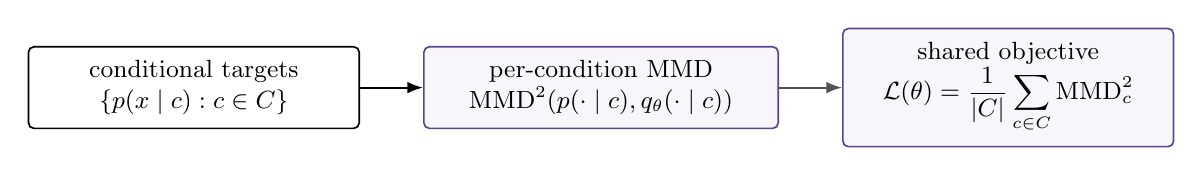
\begin{tikzpicture}[node distance=7mm and 8mm]

 \node[target,minimum width=42mm] (family)
   {conditional targets\\
    $\{p(x\mid c): c\in C\}$};

 \node[estimator,right=of family,minimum width=45mm] (per)
   {per-condition MMD\\
    $\mathrm{MMD}^2\!\left(
      p(\cdot\mid c),
      q_\theta(\cdot\mid c)
    \right)$};

 \node[estimator,right=of per,minimum width=42mm] (avg)
   {shared objective\\
    $\displaystyle
      \mathcal L(\theta)
      =
      \frac{1}{|C|}
      \sum_{c\in C}
      \mathrm{MMD}^2_c$};

 % \node[estimator,right=of avg,minimum width=25mm] (upd)
 %   {update\\
 %    $\boldsymbol\theta$};

 \draw[dataflow] (family) -- (per);
 \draw[flow]     (per)    -- (avg);
 %\draw[feedback] (avg)    -- (upd);

\end{tikzpicture}%
}

\widefigurecaption{Conditional IQP Born machine. For each condition $c_i$, an encoder prepares a classically tractable input state $\ket{\phi(c_i)}$. The same IQP unitary $U_{\theta}=H^{\otimes n}D_G(\boldsymbol\theta)H^{\otimes n}$, defined by a fixed graph $G$ and a parameter vector $\boldsymbol\theta$, is used for all conditions. The conditional family is therefore represented by varying only the input state. During training, the per-condition discrepancies $\mathrm{MMD}^2\!\left(p(\cdot\mid c), q_\theta(\cdot\mid c) \right)$ are averaged into the shared objective $\mathcal L(\theta) = |C|^{-1} \sum_{c\in C} \mathrm{MMD}^2_c$, yielding updates to a single parameter vector. }{fig:pipeline_workflow}
\end{minipage}
\end{figure*}
\section{Introduction}

Conditional generative models learn $q_\theta(x\mid c)$, a family of output distributions indexed by a condition $c$. Quantum circuit Born machines (QCBMs) represent discrete distributions through measurement statistics and can be trained with likelihood-free objectives such as maximum mean discrepancy (MMD) \cite{liuDifferentiableLearning2018,benedettiGenerativeModeling2019,gaoQuantumGenerativeModels2018}. Conditional Born machines have already been studied \cite{kissConditionalBornMachine2022,zengConditionalQCBM2023}, and input-state encoding is established in quantum circuit learning \cite{mitaraiQuantumCircuitLearning2018,schuldEffectDataEncoding2021,casasMultidimensionalFourier2023}. For an IQP model, one way to introduce a condition is to vary phases in its commuting diagonal layer. Here we impose a different sharing constraint: the graph and learned diagonal phases are identical at every condition, and only the prepared input state changes. We ask which input families preserve the classical observable estimators used to train the shared circuit.

Classical IQP training provides the starting point. IQPopt and the generative-learning framework of Recio-Armengol and collaborators estimate Pauli-$Z$ moments, express the Hamming-kernel MMD through those moments, and differentiate the resulting classical estimator \cite{recio-armengolIQPoptFastOptimization2025,recio-armengolTrainClassicalDeploy2026}. Van den Nest's computationally tractable-state framework supplies a broader foundation for estimating matrix elements of efficiently computable sparse operators \cite{nestSimulatingQuantumComputers2011}. We use this established machinery to formulate a conditional interface: for each $c$, the state entering the diagonal layer must support efficient basis sampling and evaluation of the amplitude ratios induced by the observable's bit flips. Section~\ref{sec:ratio-estimator} derives the resulting nonuniform-reference estimator, its finite-second-moment bound, and phase gradients. Section~\ref{sec:unbiased-conditional-mmd} combines it with the established U-statistic construction for MMD. The condition average trains one shared phase vector; the encoder is fixed with respect to those phases.

The contribution is this explicit sampling-and-ratio formulation of fixed-unitary conditional IQP generation, together with tractable encoder constructions and a study of their interpolation limits. The character expansion, U-statistic correction, automatic-differentiation strategy, and general input-encoding principle are inherited ingredients. The spin-flip construction extends the fixed GHZ input used in Ref.~\cite{recio-armengolTrainClassicalDeploy2026} to a condition-dependent cat-like family. Keeping the learned unitary fixed gives one parameter set that can be evaluated at a new condition without fitting a new circuit; it still requires condition-dependent state preparation. Gaussian and Curie--Weiss experiments measure the accuracy cost of this sharing constraint and its response to ancillas. A coupled-ring experiment tests two-input composition and correlated reference access beyond Hamming-shell encodings. These studies do not measure a reduction in hardware execution time. Figure~\ref{fig:pipeline_workflow} shows the separation between the encoder and the shared unitary.

Gaussian Hamming-weight targets test translation, and Curie--Weiss targets test a change in distribution shape with inverse temperature. Across both families at eight and twelve visible qubits, ancillas reduce median held-out raw bitstring TVD. The shared model improves on adjacent-independent interpolation for the ten-ancilla Gaussian model at eight visible qubits and for the ten-ancilla Curie--Weiss model at both sizes; the Gaussian comparison at twelve visible qubits remains unresolved. Curie--Weiss uses a known spin-flip symmetry and a problem-informed map containing the $\beta=1$ landmark. Its gains on the non-landmark held-out temperatures $\beta\in\{0.6,0.8,1.2,1.4\}$ support interpolation within that prescribed map. The finite-size crossover is not a measurement of critical scaling.

Two coupled periodic Ising rings provide a third, spatially structured family. At held-out combinations of two couplings, both symmetry-only and bond-informed inputs improve through a shared IQP unitary. The bond family yields lower mean joint error at both sizes, while a classical log-linear predictor remains more accurate. Encoder-only controls and output-structure diagnostics distinguish the supplied correlations from the additional learned contribution.

State conditioning therefore extends classically trained IQP Born machines from a single distribution to a condition-indexed family without reprogramming the diagonal unitary. Our evidence covers within-range interpolation on exchangeable targets and held-out combinations of two couplings on finite spatially structured rings. The Curie--Weiss experiment does not isolate the effects of the spin-flip construction and ancilla marginalization. We make no claim of universal conditional approximation, classical output sampling, quantum advantage, thermal-state preparation, or favorable optimization behavior \cite{shenCharacterizingTrainability2026}.

\section{Conditional IQP model}
Let $\mathcal{C}$ denote the condition space and let $\{p(\cdot\mid c):c\in\mathcal{C}\}$ be a family of target distributions over $n$-bit strings. We represent this family by encoding each condition $c$ in an input state $\ket{\phi(c)}$ and applying a shared parameterized IQP unitary $U_{\boldsymbol{\theta}}$. The resulting conditional model is
\begin{equation}
    q_{\boldsymbol{\theta}}(x\mid c)=\left|\bra{x}U_{\boldsymbol{\theta}}\ket{\phi(c)}\right|^2,
    \qquad x\in\{0,1\}^n .
    \label{eq:cond_sampling}
\end{equation}

The circuit graph and parameter vector are shared across the entire conditional family. We optimize $\boldsymbol{\theta}$ during training, but neither the graph nor $\boldsymbol{\theta}$ changes when the condition changes. Consequently, the model response to $c$ arises from the input state $\ket{\phi(c)}$, rather than from condition-dependent gates in the learned IQP unitary. The state-preparation circuit need not itself have IQP form; throughout this work, ``IQP unitary'' refers specifically to the shared learned unitary $U_{\boldsymbol{\theta}}$.

We define the shared IQP unitary through an undirected graph $G=(V,E)$ with $n=|V|$ vertices. Each vertex carries a one-body generator $Z_i$, and each edge $\{i,j\}\in E$ carries a two-body generator $Z_iZ_j$. For $\boldsymbol{\theta}\in\mathbb{R}^{|V|+|E|}$, the corresponding IQP unitary is
\begin{equation}
    U_{\boldsymbol{\theta}}=H^{\otimes n}D_G(\boldsymbol{\theta})H^{\otimes n},
    \label{eq:iqp-unitary}
\end{equation}
where the diagonal layer is
\begin{equation}
    D_G(\boldsymbol{\theta})=\exp\left(i\sum_{i\in V}\theta_iZ_i+i\sum_{\{i,j\}\in E}\theta_{ij}Z_iZ_j\right).
    \label{eq:graph-diagonal}
\end{equation}

All generators in $D_G(\boldsymbol{\theta})$ commute. The unitary therefore contains $|V|+|E|$ trainable phase parameters, one for each vertex and edge.

To identify conditional encoders that preserve classical estimation, let
\begin{equation}
    \psi_c(z)=\bra{z}H^{\otimes n}\ket{\phi(c)}
    \label{eq:reference-amplitude}
\end{equation}
denote the computational-basis amplitudes of the state entering the diagonal layer. Uniformly over the conditions and bit masks used by the loss, we require polynomial-time classical algorithms that sample $z$ from $|\psi_c(z)|^2$ and evaluate
\begin{equation}
    R_c(z,a)=\frac{\psi_c(z\oplus a)}{\psi_c(z)}
    \label{eq:amplitude-ratio}
\end{equation}
to the numerical precision required by the estimator.

The ratio need only be defined on the support of $|\psi_c|^2$. Computationally tractable states in the sense of Van den Nest, which permit efficient basis sampling and individual amplitude evaluation, provide a sufficient condition under exact or suitably controlled arithmetic \cite{nestSimulatingQuantumComputers2011}. Our estimator uses the narrower sampling-and-ratio interface above. For a polynomial-size IQP diagonal and a loss with an efficient Pauli-moment description, these operations yield polynomial-time additive estimators of the Pauli-$Z$ moments used for training \cite{recio-armengolIQPoptFastOptimization2025,recio-armengolTrainClassicalDeploy2026}. Section~\ref{sec:ratio-estimator} derives the estimator and its finite-second-moment guarantee. This access does not provide exact output probabilities or efficient classical samples from $q_{\boldsymbol{\theta}}(x\mid c)$.

\subsection{Product-state conditioning}
Product states provide a direct realization of the tractability interface above. We assign each qubit a fixed rotation axis $j_i\in\{X,Y\}$ and encode the condition through the rotation angles,
\begin{equation}
    \ket{\phi(c)}=\bigotimes_{i=1}^{n}R_{j_i}\!\left(\alpha_i(c)\right)\ket{0}.
    \label{eq:product-encoder}
\end{equation}

The physical meaning and normalization of $c$ depend on the target family. The axes $j_i$ and angle maps $\alpha_i$ are fixed before training; changing the condition changes only the prepared input state and leaves the shared IQP parameters $\boldsymbol{\theta}$ unchanged.

The local Hadamards before the diagonal layer preserve this product structure. Define $\ket{\chi_i(c)}=H R_{j_i}(\alpha_i(c))\ket{0}$ and $\psi_{c,i}(b)=\braket{b|\chi_i(c)}$ for $b\in\{0,1\}$. The reference amplitudes in Eq.~\eqref{eq:reference-amplitude} then factorize as
\begin{equation}
    \psi_c(z)=\prod_{i=1}^{n}\psi_{c,i}(z_i).
    \label{eq:product-amplitudes}
\end{equation}

Consequently, we can sample each bit $z_i$ independently from $|\psi_{c,i}(z_i)|^2$. For every sampled string and every mask $a$, the ratio in Eq.~\eqref{eq:amplitude-ratio} is
\begin{equation}
    R_c(z,a)=\prod_{i:a_i=1}\frac{\psi_{c,i}(1-z_i)}{\psi_{c,i}(z_i)}.
    \label{eq:product-amplitude-ratio}
\end{equation}

Both operations require at most $O(n)$ single-qubit evaluations, so this encoder satisfies the sampling-and-ratio interface uniformly over $c$ and $a$, subject to the numerical-precision requirement stated above. If every angle map is affine, $\alpha_i(c)=\omega_i c+\beta_i$, each output probability is a finite Fourier series in $c$ whose frequencies are signed sums of the encoding frequencies $\omega_i$ \cite{schuldEffectDataEncoding2021,casasMultidimensionalFourier2023}.

\subsection{Symmetry-informed conditioning}

The zero-field Curie--Weiss distribution is invariant under a global spin flip at every inverse temperature $\beta$,
\begin{equation}
    p_\beta(x)=p_\beta(\bar{x}),
    \label{eq:curie-spin-flip-target}
\end{equation}
where $\bar{x}$ flips every bit in $x$. This is a within-condition symmetry: the transformation changes the spin configuration but leaves $\beta$ fixed.

Recio-Armengol, Ahmed, and Bowles showed that a GHZ input enforces this global bit-flip invariance in an IQP-structured Born machine while retaining a classical estimator for the observables required during training \cite{recio-armengolTrainClassicalDeploy2026}. We use the same symmetry principle, but replace their fixed unconditional GHZ input with a condition-dependent family of spin-flip-symmetrized states. Let $m$ denote the size of the register on which the encoder acts and let $F_m=X^{\otimes m}$.

Define the broadcast product state
\begin{equation}
    \ket{p_{\alpha(\beta)}}^{\otimes m}
    =\left[R_Y\!\left(\alpha(\beta)\right)\ket{0}\right]^{\otimes m}.
    \label{eq:curie-base-product-state}
\end{equation}
Our Curie--Weiss encoder is
\begin{equation}
    \ket{\phi_{\mathrm{sf}}^{(m)}(\beta)}
    =\frac{\ket{p_{\alpha(\beta)}}^{\otimes m}+F_m\ket{p_{\alpha(\beta)}}^{\otimes m}}{\sqrt{\mathcal N_\beta}},
    \label{eq:spin-flip-encoder}
\end{equation}
where $\mathcal N_\beta$ is the normalization factor. Equation~\eqref{eq:spin-flip-encoder} is a condition-dependent cat-like state. It reduces to the GHZ construction of Ref.~\cite{recio-armengolTrainClassicalDeploy2026} when $\alpha(\beta)=0$.

The encoder satisfies $F_m\ket{\phi_{\mathrm{sf}}^{(m)}(\beta)}=\ket{\phi_{\mathrm{sf}}^{(m)}(\beta)}$. Moreover, every generator of the IQP unitary in the $X$ basis commutes with $F_m$, and hence $[U_{\boldsymbol{\theta}}^{(m)},F_m]=0$. Its $m$-bit output distribution therefore obeys
\begin{equation}
    q_{\boldsymbol{\theta}}^{(m)}(y\mid\beta)
    =q_{\boldsymbol{\theta}}^{(m)}(\bar{y}\mid\beta).
    \label{eq:register-spin-flip-invariance}
\end{equation}

The symmetry condition alone does not establish classical tractability. For the state in Eq.~\eqref{eq:spin-flip-encoder}, however, the amplitudes entering the diagonal layer depend only on the Hamming weight. Write $c_\beta=\cos[\alpha(\beta)/2]$, $s_\beta=\sin[\alpha(\beta)/2]$, $u_\beta=(c_\beta+s_\beta)/\sqrt{2}$, and $v_\beta=(c_\beta-s_\beta)/\sqrt{2}$. For a string $z$ of weight $k=|z|$,
\begin{equation}
    \psi_\beta(z)=A_\beta(k)
    =\frac{u_\beta^{m-k}v_\beta^k\left[1+(-1)^k\right]}{\sqrt{\mathcal N_\beta}}.
    \label{eq:spin-flip-shell-amplitude}
\end{equation}
Odd-weight amplitudes vanish, while all strings within an even-weight shell have the same amplitude. We sample the reference state by first drawing an even weight $k$ with probability
\begin{equation}
    P_\beta(k)=\binom{m}{k}|A_\beta(k)|^2
    \label{eq:spin-flip-shell-probability}
\end{equation}
and then drawing a string uniformly from that shell. The amplitude ratio required by Eq.~\eqref{eq:amplitude-ratio} is obtained from the same $m+1$ shell table,
\begin{equation}
    R_\beta(z,a)=\frac{A_\beta(|z\oplus a|)}{A_\beta(|z|)}.
    \label{eq:spin-flip-shell-ratio}
\end{equation}
The denominator is nonzero for every sampled $z$. Sampling and ratio evaluation are therefore polynomial in $m$, so this condition-dependent extension retains the classical training interface. It does not imply efficient classical sampling from the trained IQP output distribution.

\subsection{Correlated two-ring conditioning}
\label{sec:two-ring-encoding}

Vector-valued conditions can enter different factors of a correlated input. For $n=2m$ qubits arranged in two layers, let $\boldsymbol c=(a,b)$. We compare a product of two normalized cat states of the form in Eq.~\eqref{eq:spin-flip-encoder}, with one angle per layer, against
\begin{equation}
 \ket{\phi_{\rm bond}(a,b)}=\ket{B_a}\otimes\ket{B_b},\qquad
 \langle x|B_g\rangle=\frac{e^{(g/2+i\eta)E(x)}}{\sqrt{Z_m(g)}},
 \label{eq:bond-input}
\end{equation}
where $E(x)=\sum_{i=0}^{m-1}(1-2x_i)(1-2x_{i+1})$, indices are periodic, $Z_m(g)=(2\cosh g)^m+(2\sinh g)^m$, and $\eta=\pi/8$ is fixed. The bond-informed input supplies the uncoupled within-layer Ising law and its coupling dependence; it supplies no interlayer dependence. The symmetry-only cat input supplies the layer partition and its prescribed angle map. Neither input is prior-free.

Both inputs are fixed by independent global flips of either layer. These flips commute with $U_{\boldsymbol\theta}$, so both outputs enforce $\mathbb Z_2\times\mathbb Z_2$ invariance for every phase vector, including with interlayer generators. The unrestricted phase bank does not enforce ring translations or reflections. The coupled-ring target is covariant under exchanging the layers and $(a,b)$ together; we do not impose that covariance on the learned circuit.

The bond reference entering the diagonal layer need not have Hamming-shell amplitudes. Define $T_{uv}=\exp[(g/2+i\eta)(1-2u)(1-2v)]$ and $A_z=\operatorname{diag}(1,(-1)^z)T$. Its amplitudes are
\begin{equation}
 \psi_g(z)=\frac{\operatorname{tr}(A_{z_0}\cdots A_{z_{m-1}})}{\sqrt{2^m Z_m(g)}}.
 \label{eq:bond-transfer-amplitude}
\end{equation}
Thus amplitude ratios use $2\times2$ contractions, while reference sampling uses $4\times4$ doubled contractions. Each amplitude query or draw requires $O(m)$ arithmetic, with $O(m)$ suffix preparation for sampling. Appendix~\ref{app:at-reference} derives the sampler and a coherent preparation construction, and states their precision and routing assumptions. This provides a correlated realization of the same sampling-and-ratio interface, rather than a new training estimator.

\subsection{Ancilla-assisted conditioning}

Ancillas extend any of the preceding encoders while retaining a visible $n$-bit output. Let $r$ denote the number of ancillas and $N=n+r$ the size of the joint register. We prepare an $N$-qubit state $\ket{\Phi(c)}$, apply $U_{\boldsymbol{\theta}}^{(N)}$, and marginalize the ancillary outcomes,
\begin{equation}
    q_{\boldsymbol{\theta}}(x\mid c)=\sum_{a\in\{0,1\}^{r}}\left|\bra{x,a}U_{\boldsymbol{\theta}}^{(N)}\ket{\Phi(c)}\right|^2.
    \label{eq:ancilla-visible-marginal}
\end{equation}
For the scalar product encoder in Eq.~\eqref{eq:product-encoder}, the tensor product runs over $N$ rather than $n$ qubits and may retain qubit-dependent axes and angle maps. For the spin-flip encoder in Eq.~\eqref{eq:spin-flip-encoder}, we set $m=N$; unlike the product construction, this state is a coherent superposition and requires the shell-based sampler and ratio evaluator above. In these two constructions, the ancillas receive the condition rather than entering as condition-independent workspace.

For the spin-flip construction, Eq.~\eqref{eq:register-spin-flip-invariance} gives $q_{\boldsymbol{\theta}}(x,a\mid\beta)=q_{\boldsymbol{\theta}}(\bar{x},\bar{a}\mid\beta)$ on the joint register. Summing over $a$ and relabelling $a\mapsto\bar{a}$ preserves the symmetry after marginalization,
\begin{equation}
    q_{\boldsymbol{\theta}}(x\mid\beta)
    =q_{\boldsymbol{\theta}}(\bar{x}\mid\beta).
    \label{eq:visible-spin-flip-invariance}
\end{equation}

Although the joint output is pure, tracing out the ancillas can produce a mixed visible state of rank at most $2^r$. Kurkin et al. prove that, for unrestricted parameterized IQP Born machines, $n+1$ hidden qubits suffice for exact distributional universality on $n$ visible bits \cite{kurkinUniversalityKernelAdaptive2025}. Their construction may require exponentially many diagonal terms. We do not claim that our two-local model is universal.

The complete two-local bank stores $P_N=N+\binom{N}{2}$ phase coordinates, but not all affect visible outputs. Any ancilla-only diagonal factor commutes through the other diagonal gates and becomes a local ancillary unitary after the final Hadamards; it cancels under the partial trace for any input, including an entangled one. Equivalently, its $d_{j,a}$ in Eq.~\eqref{eq:conditional-phase-gradient} vanishes for every visible mask. Removing the $r(r+1)/2$ ancilla-only coordinates leaves at most $n+\binom n2+nr$ visible-affecting phase directions, before any additional encoder-induced redundancies. The frozen Gaussian and Curie--Weiss runs retain the full stored bank. The Ashkin--Teller ancilla follow-up omits these inactive coordinates. Visible--ancilla couplings and the condition-dependent joint input can still change visible predictions; affine product encodings can access higher signed sums of encoding frequencies as $r$ increases \cite{schuldEffectDataEncoding2021,casasMultidimensionalFourier2023}. Thus the original ancilla ladder changes both the visible model family and its supplied condition response, whose effects are not isolated.

Classical estimation still uses only visible observables. A visible Pauli mask $a\in\{0,1\}^n$ is extended to $(a,0^r)$, corresponding to $Z_a\otimes I^{\otimes r}$ on the joint register. Training remains classically estimable whenever the $N$-qubit reference state supports the sampling-and-ratio interface. The product encoder satisfies it by factorization; the spin-flip encoder satisfies it through Eqs.~\eqref{eq:spin-flip-shell-probability} and \eqref{eq:spin-flip-shell-ratio}.

\section{Conditional IQP training}
\label{sec:cond_training}

\subsection{Conditional Pauli estimator and phase gradients}
\label{sec:ratio-estimator}

Work on the joint register of $N=n+r$ qubits, with $r=0$ allowed. Write $D_{\boldsymbol\theta}\ket z=e^{if_{\boldsymbol\theta}(z)}\ket z$, where $f_{\boldsymbol\theta}(z)=\sum_{j=1}^{P_N}\theta_j\chi_{g_j}(z)$ and $g_j\in\bits^N$ is the mask of the $j$th diagonal Pauli generator, with $\chi_g(z)=(-1)^{g\cdot z}$. For a visible mask $a$, let $\widetilde a=(a,0^r)$ and $\psi_c(z)=\bra z H^{\otimes N}\ket{\Phi(c)}$. Define
\begin{equation}
\begin{aligned}
    \Delta_a f_{\boldsymbol\theta}(z)
      &=f_{\boldsymbol\theta}(z\oplus\widetilde a)-f_{\boldsymbol\theta}(z),\\
    W_{c,a}(z;\boldsymbol\theta)
      &=R_c(z,\widetilde a)e^{i\Delta_a f_{\boldsymbol\theta}(z)},\\
    Y_{c,a}(z;\boldsymbol\theta)&=\operatorname{Re}W_{c,a}(z;\boldsymbol\theta).
\end{aligned}
\label{eq:ratio-sample}
\end{equation}
Conjugating $Z_a\otimes I^{\otimes r}$ through the final Hadamards gives $X_{\widetilde a}$. Expanding its expectation before the diagonal layer therefore yields
\begin{equation}
\begin{aligned}
    \mu_q(a\mid c)
    &=\bra{\psi_c}D_{\boldsymbol\theta}^{\dagger}
      X_{\widetilde a}D_{\boldsymbol\theta}\ket{\psi_c}\\
    &=\sum_z\psi_c(z)^*\psi_c(z\oplus\widetilde a)
       e^{i\Delta_a f_{\boldsymbol\theta}(z)}\\
    &=\E_{z\sim|\psi_c|^2}[Y_{c,a}(z;\boldsymbol\theta)].
\end{aligned}
\label{eq:conditional-pauli-estimator}
\end{equation}
The expectation is real because the observable is Hermitian. For the uniform reference state, $R_c=1$ and Eq.~\eqref{eq:conditional-pauli-estimator} reduces to the cosine estimator used in IQPopt \cite{recio-armengolIQPoptFastOptimization2025}. The ratio is the additional factor needed for the conditional reference state.

\begin{proposition}[Finite-variance conditional estimation]
For a normalized reference state satisfying the sampling-and-ratio interface and a polynomial-size diagonal generator list, a visible Pauli moment and any one of its phase derivatives admit classical additive-error estimates with $O(\epsilon^{-2}\log(1/\delta))$ reference samples, to error $\epsilon$ and failure probability at most $\delta$. The encoder is independent of $\boldsymbol\theta$. The statement assumes exact reference sampling, with exact arithmetic or the controlled evaluation errors specified below.
\end{proposition}
\begin{proof}
On the support $S_c=\{z:\psi_c(z)\ne0\}$,
\begin{equation}
\begin{aligned}
    \E|W_{c,a}|^2
    &=\sum_{z\in S_c}|\psi_c(z\oplus\widetilde a)|^2\leq1,\\
    \operatorname{Var}(Y_{c,a})&\leq\E[Y_{c,a}^2]\leq1.
\end{aligned}
\label{eq:ratio-second-moment}
\end{equation}
No full-support assumption is needed. Zero numerators contribute zero, and zero denominators are never sampled. Since the sampling law and ratio do not depend on the learned phases, differentiation gives
\begin{equation}
\begin{aligned}
    d_{j,a}(z)&=\chi_{g_j}(z\oplus\widetilde a)-\chi_{g_j}(z),\\
    \partial_{\theta_j}\mu_q(a\mid c)
      &=\E[\operatorname{Re}(i\,d_{j,a}W_{c,a})].
\end{aligned}
\label{eq:conditional-phase-gradient}
\end{equation}
Here $d_{j,a}\in\{-2,0,2\}$, so the derivative sample has second moment at most $4$. Sample means consequently attain constant-success additive accuracy with $O(\epsilon^{-2})$ draws by Chebyshev's inequality; a median of independent block means gives failure probability $\delta$ with $O(\log(1/\delta))$ blocks. Each sample requires polynomial work under the stated interface.
\end{proof}

Individual ratios can be large, so bounded-sample concentration does not apply directly. The proposition is a finite-variance guarantee; production uses ordinary sample means rather than median-of-means aggregation. Conditions, encoders, and generator lists must have polynomial-size descriptions, and the interface must be efficient uniformly over the requested conditions and masks. For numerical evaluation, it suffices that the computed $W_{c,a}$ has root-mean-square error $\eta$ under the reference law, achievable in polynomial time at the requested precision: the moment bias is then at most $\eta$ and the phase-derivative bias at most $2\eta$. Choosing $\eta=O(\epsilon)$ preserves additive accuracy. An approximate sampler requires a separate bias bound for these potentially unbounded ratio-weighted observables; a small total-variation sampling error alone is insufficient. Approximate amplitude queries alone do not establish this requirement when denominators are small. These estimates concern fixed encoders and additive phase-gradient accuracy; they do not establish efficient optimization or cover learned encoder parameters that change the reference sampling law.

\subsection{Condition-balanced MMD objective}

We train the shared circuit with the squared maximum mean discrepancy (MMD) \cite{grettonKernelTwoSample2012}. For two distributions $p$ and $q$ on $\bits^n$ and a positive-definite kernel $k$, the population discrepancy is
\begin{equation}
\begin{aligned}
\mmd^2(p,q)={}&\E_{x,x'\sim p}[k(x,x')]
  -2\E_{x\sim p,\,y\sim q}[k(x,y)]\\
  &+\E_{y,y'\sim q}[k(y,y')].
\end{aligned}
\label{eq:mmd-population}
\end{equation}

On binary strings, we use the Hamming radial basis function kernel
\begin{equation}
    k_\sigma(x,y)=\exp\!\left[-\frac{d_H(x,y)}{2\sigma^2}\right],
    \label{eq:hamming-rbf-kernel}
\end{equation}
where $d_H$ is the Hamming distance and $\sigma>0$ is the bandwidth.

Let $\mathcal C_{\mathrm{train}}$ denote the training conditions and $\Sigma$ the bandwidth set. We assign equal weight to every condition and bandwidth,
\begin{equation}
\mathcal{L}(\boldsymbol\theta)=\frac{1}{|\mathcal C_{\mathrm{train}}|}
\sum_{c\in\mathcal C_{\mathrm{train}}}\frac{1}{|\Sigma|}
\sum_{\sigma\in\Sigma}\mmd^2_\sigma\!\left(p(\cdot\mid c),
q_{\boldsymbol\theta}(\cdot\mid c)\right).
\label{eq:conditional-objective}
\end{equation}
Equal condition weighting prevents differences in sample availability from changing the relative influence of each condition on the shared parameter vector. For fixed parameters and independent target and reference draws, the U-statistic construction below replaces the population moments by unbiased estimates. The production procedure reuses frozen datasets and mask banks, as distinguished below.

\subsection{Character expansion and bandwidth coverage}

The Hamming-RBF kernel has a product character representation. Let $a\in\bits^n$ be a visible-bit mask with independent coordinates
\begin{equation}
    a_i\sim\operatorname{Bernoulli}(p_\sigma),
    \qquad
    p_\sigma=\frac{1-e^{-1/(2\sigma^2)}}{2},
    \label{eq:mmd-mask-law}
\end{equation}
and define the binary character $\chi_a(x)=(-1)^{a\cdot x}$. Then
\begin{equation}
    k_\sigma(x,y)=\E_a\!\left[\chi_a(x)\chi_a(y)\right].
    \label{eq:hamming-character-expansion}
\end{equation}
If $\mu_p(a)=\E_{x\sim p}[\chi_a(x)]$, substituting Eq.~\eqref{eq:hamming-character-expansion} into Eq.~\eqref{eq:mmd-population} gives
\begin{equation}
    \mmd_\sigma^2(p,q)=
    \E_a\!\left[\left(\mu_p(a)-\mu_q(a)\right)^2\right].
    \label{eq:mmd-character-moments}
\end{equation}
For the Born machine, $\mu_q(a)$ is the expectation value of the visible Pauli string $Z_a=\bigotimes_i Z_i^{a_i}$. Equation~\eqref{eq:mmd-character-moments} is therefore the link between the conditional MMD and the classically estimated observables described above \cite{recio-armengolIQPoptFastOptimization2025,recio-armengolTrainClassicalDeploy2026}.

The mask weight $K=|a|$, also called the operator bodyness, follows a binomial distribution,
\begin{equation}
    \begin{aligned}
        K&\sim\operatorname{Binomial}(n,p_\sigma),\\
        \E[K]&=np_\sigma,
        &\operatorname{Var}(K)&=np_\sigma(1-p_\sigma).
    \end{aligned}
    \label{eq:mmd-bodyness-distribution}
\end{equation}
Thus, a bandwidth controls a distribution over correlation orders rather than selecting one order. Large bandwidths favor low-weight observables, while decreasing $\sigma$ shifts mass toward higher weights. The mean approaches $n/2$ as $\sigma\rightarrow0$. Within a fixed weight, the isotropic kernel assigns the same coefficient to every mask.

We use three bandwidths whose target mean mask weights are
\begin{equation}
    \bar K_1=1,
    \qquad
    \bar K_2=\frac{1+0.49n}{2},
    \qquad
    \bar K_3=0.49n,
    \label{eq:mmd-target-bodyness}
\end{equation}
with
\begin{equation}
    \sigma(\bar K)=
    \left[-2\log\!\left(1-\frac{2\bar K}{n}\right)\right]^{-1/2}.
    \label{eq:mmd-bodyness-to-sigma}
\end{equation}
The first bandwidth emphasizes low-order correlations, the third approaches the largest mean weight available to this isotropic family, and the second lies between them. We apply this fixed rule at every visible-system size and for every dataset to broaden coverage of correlation orders that may contribute to the target--model residual. We do not claim that these bandwidths are optimal. Dataset-specific or residual-adaptive kernel selection could improve the training signal, but it lies outside the scope of this work.

\subsection{Unbiased squared moments and loss gradients}
\label{sec:unbiased-conditional-mmd}

Fix a condition, visible mask, and parameter vector. Let $T_b=\chi_a(x_b)$ for $B\geq2$ independent target samples and let $Y_s=Y_{c,a}(z_s;\boldsymbol\theta)$ for $S\geq2$ independent reference samples, drawn independently of the target samples. With $\overline T=B^{-1}\sum_b T_b$ and $\overline Y=S^{-1}\sum_sY_s$, define
\begin{equation}
\begin{aligned}
    \widehat{\Delta^2}(a)
    ={}&\frac{(\sum_sY_s)^2-\sum_sY_s^2}{S(S-1)}
       -2\overline Y\,\overline T\\
       &+\frac{(\sum_bT_b)^2-B}{B(B-1)}.
\end{aligned}
\label{eq:conditional-mmd-ustatistic}
\end{equation}
The first and last terms average products over distinct sample indices, so their expectations are $\mu_q(a)^2$ and $\mu_p(a)^2$. The cross term has expectation $-2\mu_q(a)\mu_p(a)$. Thus $\E\widehat{\Delta^2}(a)=(\mu_q(a)-\mu_p(a))^2$. This is the U-statistic correction used for IQP MMD training \cite{recio-armengolTrainClassicalDeploy2026}, here applied to the ratio-weighted real samples. Squaring $\overline Y$ alone would add $\operatorname{Var}(Y)/S$. An unbiased finite-sample estimate can be negative.

Writing $Y'_s=\partial_{\theta_j}Y_s$ from Eq.~\eqref{eq:conditional-phase-gradient}, differentiation of the same expression gives
\begin{equation}
    \partial_{\theta_j}\widehat{\Delta^2}(a)
    =\frac{2\sum_{s\ne t}Y_sY'_t}{S(S-1)}
       -2\overline T\,\overline{Y'}.
\label{eq:conditional-mmd-gradient}
\end{equation}
Independence across reference draws makes its expectation $2(\mu_q-\mu_p)\partial_{\theta_j}\mu_q$. The diagonal subtraction is essential because $Y_s$ and $Y'_s$ from the same draw can be correlated. Automatic differentiation with the sampled strings held fixed computes Eq.~\eqref{eq:conditional-mmd-gradient}; no derivative of the sampler is needed for the learned phases.

The second-moment bounds also suffice for the loss and each gradient component. For independent copies $(Y,T)$ and $(\widetilde Y,\widetilde T)$, the pair kernel $(Y-T)(\widetilde Y-\widetilde T)$ has second moment at most $16$, since $\E(Y-T)^2\leq4$. Its phase derivative has second moment at most $64$, using $\E(Y')^2\leq4$. Equation~\eqref{eq:conditional-mmd-ustatistic} averages the corresponding distinct-index products. Thus finite variance requires no fourth-moment bound on an individual ratio. Efficient mask sampling and condition averaging preserve polynomial-cost additive estimation; simultaneous componentwise control of all $P_N$ gradients can use a union bound with per-component failure probability $\delta/P_N$.

\subsection{Stochastic operator estimator}

The identity mask has $\mu_p(0)=\mu_q(0)=1$ and therefore contributes zero to Eq.~\eqref{eq:mmd-character-moments}. We sample only nonidentity masks from the conditional law $P_\sigma(a\mid a\ne0)$. Its total nonidentity mass is
\begin{equation}
    Q_\sigma^+=1-(1-p_\sigma)^n.
    \label{eq:mmd-nonidentity-mass}
\end{equation}
Multiplying the conditional sample average by $Q_\sigma^+$ preserves the original Hamming-RBF objective. If $M$ mask draws contain a set $\mathcal U$ of unique masks and mask $u$ occurs $m_u$ times, the estimator can be written as
\begin{equation}
    \widehat{\mmd}_\sigma^2
    =Q_\sigma^+\sum_{u\in\mathcal U}\frac{m_u}{M}
    \widehat{\Delta^2}(u),
    \label{eq:compressed-mmd-estimator}
\end{equation}
where $\widehat{\Delta^2}(u)$ is given by Eq.~\eqref{eq:conditional-mmd-ustatistic}. Combining duplicates changes neither the sampled objective nor its gradient; it avoids evaluating the same Pauli observable more than once.

For fixed parameters, averaging also over the sampled mask bank recovers the full kernel objective. In production, each condition--bandwidth mask bank is drawn once per fit and retained, while reference strings are resampled during training. Conditional on that bank, the reference estimator targets the finite weighted mask objective. Likewise, the target U-statistic is population-unbiased for independent data at fixed parameters; repeatedly using a frozen dataset does not make the gradients along an adaptive optimization trajectory independent population estimates. Correlations from reusing reference strings across masks do not change the fixed-parameter expectation.

For every finite $\sigma$, the exact kernel assigns positive weight to every character and is characteristic on the finite hypercube. This identifiability at fixed dimension does not imply that polynomial-precision MMD controls TVD uniformly as dimension grows \cite{kurkinUniversalityKernelAdaptive2025}. The finite operator and state-sampling budgets still limit coverage and introduce estimator variance. We use MMD as the differentiable optimization loss and exact visible-distribution TVD for scientific evaluation. Gaussian and Curie--Weiss checkpoints are selected by exact validation TVD; the separately frozen Ashkin--Teller study uses sampled validation MMD (Sec.~\ref{sec:at-protocol}).

\subsection{Computational and sample complexity}
\label{sec:estimator-complexity}

Let $A=|\mathcal U|$ be the number of distinct masks, $P=P_N$ the number of diagonal generators, and $L_g=\sum_{j=1}^{P}|g_j|$ their total support size. We count arithmetic operations at fixed or controlled precision, excluding compilation. Table~\ref{tab:reference-cost} gives the reference costs for one condition. All three families admit linear-time preprocessing and linear-time ratio queries for arbitrary masks; their constants and sampling procedures differ. The bounds cover the single symmetrized input and a fixed number of independent blocks, including the two-block Ashkin--Teller inputs.

\begin{table}[tb]
\caption{Reference-interface operation counts for $N$ qubits. Sampling cost $T_s(N)$ is per string after preprocessing; ratio cost is per string--mask pair. The symmetry-only row counts the sorting-based sampler used here. A sequential uniform fixed-weight sampler can instead attain $O(N)$ per string.}
\label{tab:reference-cost}
\centering
\begin{tabular}{lccc}
\toprule
Reference & Setup & $T_s(N)$ & Ratio \\
\midrule
Product & $O(N)$ & $O(N)$ & $O(N)$ \\
Symmetry-only & $O(N)$ & $O(N\log N)$ & $O(N)$ \\
Bond-informed & $O(N)$ & $O(N)$ & $O(N)$ \\
\bottomrule
\end{tabular}
\end{table}

For product inputs, sampling uses independent Bernoulli draws and a ratio is a product of local factors. For symmetry-only inputs, we first sample the Hamming weight in each block, then a uniform string of that weight; two sorts implement the latter step. Ratios follow from the original and flipped block weights. Bond-informed inputs use $N$ contractions of constant-size transfer matrices for sampling and amplitude queries. For a mask of weight $w$, product and symmetry-only ratios can be evaluated in $O(1+w)$ after caching the original block weights and using a support-list representation; the implementation uses dense masks.

Generator characters can be computed from their supports in $O(L_g)$ per reference string. The mask--generator flip indicators require $O(AL_g)$ preprocessing. Reusing both across observables, $S$ draws give all $A$ moments and, by Eq.~\eqref{eq:conditional-phase-gradient}, their full $A\times P$ phase Jacobian in attainable time
\begin{equation}
\begin{aligned}
    T_{\mathrm{mom,J}}=O\bigl(&N+AL_g\\
      &+S[T_s(N)+L_g+A(N+P)]\bigr).
\end{aligned}
\label{eq:estimator-batched-cost}
\end{equation}
The Jacobian accumulation costs $O(SAP)$: each phase derivative reuses the already computed ratio and phase. It does not require $P$ new reference samples or circuit evaluations. Streaming over reference strings gives an attainable memory bound $O(N+L_g+AN+AP)$, including the mask bank and Jacobian output. With all one- and two-body generators, $P=\Theta(N^2)$ and $L_g=\Theta(N^2)$, so Eq.~\eqref{eq:estimator-batched-cost} is $O(SAN^2)$ for each of the three families, for $S,A\geq1$. This is an algorithmic bound, not a fit to wall-clock measurements.

The current vectorized implementation does not realize every saving in Eq.~\eqref{eq:estimator-batched-cost}. Its dense parity products give the forward operation count
\begin{equation}
\begin{aligned}
    T_{\mathrm{dense}}=O\bigl(&N+(S+A)NP\\
      &+SAP+SAN+ST_s(N)\bigr).
\end{aligned}
\label{eq:estimator-dense-cost}
\end{equation}
The $ANP$ mask preprocessing can be reused. Scalar loss differentiation has the same leading arithmetic order as its forward computation. In contrast, the benchmark harness constructs a full vector-output Jacobian with reverse-mode automatic differentiation: its compiled product-input programs contain an $A\times A\times S$ intermediate and an $A^2\times S$ by $S\times P$ contraction. That path incurs $O(SA^2P)$ work, rather than the attainable $O(SAP)$ analytic accumulation. At fixed $A$, the dense parity term yields the conservative bound $O(SN^3)$ for the complete one-/two-body bank. Compilation time and compiler fusion are separate implementation properties; neither is an asymptotic estimator bound.

For the MMD loss, target characters cost $O(ABn)$ for $B$ examples on $n$ visible bits. The squared-sum identities in Eq.~\eqref{eq:conditional-mmd-ustatistic} add only $O(A(S+B))$ work, avoiding explicit $S^2$ and $B^2$ pair loops. A scalar loss and its full phase gradient therefore cost $O(T_{\mathrm{mom,J}}+ABn)$ with support-based evaluation, or $O(T_{\mathrm{dense}}+ABn)$ in the dense implementation. Processing $C$ conditions and $H$ bandwidths multiplies these bounds by $CH$ if each bank has at most $A$ distinct masks; preprocessing and fixed target terms can be reused where applicable.

The finite-variance bounds give $S=O(\epsilon^{-2}\log(A(P+1)/\delta))$ for simultaneous componentwise accuracy $\epsilon$ of a fixed bank's moments and phase derivatives using median-of-means and a union bound. This is not an $\ell_2$-error guarantee for the whole Jacobian, nor the confidence construction used for the empirical sample means. The independent-pair loss estimator likewise has scalar additive sample complexity $O(\epsilon^{-2}\log(1/\delta))$, or a $\log(P/\delta)$ factor for simultaneous gradient components, when averaging over the required mask/condition law. Increasing $S$ with a frozen mask bank does not remove mask-bank error.

For comparison, exact enumeration can evaluate the reference amplitudes, diagonal phases and Walsh--Hadamard transforms in $O(2^N(N+L_g))$ time for these inputs. All output characters can then be obtained by a further $O(N2^N)$ transform of the probabilities, with $O(A)$ lookup cost. Streaming one phase derivative at a time gives an attainable full-Jacobian cost $O(2^N[L_g+PN]+AP)$ and memory $O(2^N+L_g+AN+AP)$. These exponential reference calculations are confined to small-system verification and evaluation; the sampled estimators do not require them.


\subsection{Balanced updates and checkpoint selection}

This subsection specifies the Gaussian and Curie--Weiss production schedule. Ashkin--Teller retains the condition-balanced objective but uses the smaller training budget and MMD selection rule in Sec.~\ref{sec:at-protocol}.

At update $t$, we draw a minibatch $\mathcal B_{c,t}$ of 100 examples from every training condition and evaluate all three bandwidths. The loss for the single shared parameter vector is
\begin{equation}
    \widehat{\mathcal L}_t(\boldsymbol\theta)
    =\frac{1}{|\mathcal C_{\mathrm{train}}|}
    \sum_{c\in\mathcal C_{\mathrm{train}}}
    \frac{1}{|\Sigma|}
    \sum_{\sigma\in\Sigma}
    \widehat{\mmd}_{\sigma,t}^2(c).
    \label{eq:balanced-training-update}
\end{equation}
We shuffle the 1,000 examples for each condition independently and traverse them without replacement. Thus, ten updates constitute one epoch, and 2,000 updates correspond to 200 epochs. Each independent baseline follows the same schedule using samples from its single condition.

We optimize Eq.~\eqref{eq:balanced-training-update} with Adam using $\beta_1=0.9$, $\beta_2=0.999$, and a cosine learning-rate schedule from $10^{-2}$ to $10^{-3}$. A preregistered comparison with schedule-free AdamW did not satisfy the adoption criterion, so we retained Adam for all production runs.

We save candidate checkpoints after 500, 1,000, 1,500, and 2,000 updates, together with the checkpoint attaining the lowest validation MMD. Among these candidates, we select the checkpoint with the lowest mean exact validation TVD. For the shared model, validation and checkpoint selection use training conditions only; held-out conditions enter neither initialization, training, nor model selection.

\section{Experimental Setup}

The following scalar-family configuration applies to Gaussian and Curie--Weiss experiments. The separately frozen Ashkin--Teller study uses the protocol in Sec.~\ref{sec:at-protocol}; it first addresses encoder structure, then crosses data size with ancilla count in Sec.~\ref{sec:data-ancilla-followup}.

\subsection{Condition encoding}

For experiments using the product-state encoder, we normalize the physical condition to $c\in[0,1]$, use $R_Y$ rotations on every circuit qubit, including the ancillas, and set
\begin{equation}
    \alpha_i(c)=\pi(0.35-0.70c),\qquad i=1,\ldots,N.
    \label{eq:experimental-angle-map}
\end{equation}

This fixed affine map centers the encoded interval at zero and gives it an angular span of $0.70\pi$. We did not optimize the map or compare it with alternative encodings, so we treat it as an implementation choice rather than an optimality claim. The production Curie--Weiss experiment instead uses the symmetry-informed encoder defined above.

We use a $2\times2$ development ablation to separate the spin-flip input from the condition map. The input is either the broadcast product state or the spin-flip state in Eq.~\eqref{eq:spin-flip-encoder}. The generic map, $\alpha_{\mathrm{gen}}(\beta)=\pi[0.125+0.25(\beta-0.5)]$, is affine on $\beta\in[0.5,1.5]$ and has no feature at $\beta=1$. The informed map is continuous and piecewise linear. At $\beta=0.5$, $0.9$, $1.0$, $1.2$, and $1.5$, its values $\alpha/\pi$ are $-0.14$, $-0.07$, $0$, $0.08$, and $0.14$, respectively. We cross these choices with $r\in\{0,10\}$ at $n=8$ and use matched seeds 100--102, giving 24 fits under the same data, training, checkpoint-selection, and exact-evaluation protocol as the production campaign. Held-out temperatures enter neither training nor checkpoint selection.

\subsection{Benchmark distributions}

\subsubsection{Discrete Gaussian family}

The Gaussian benchmark tests whether one shared circuit can follow a translated family of unimodal distributions. For a bit string $x\in\{0,1\}^n$, let $K(x)=\sum_{i=1}^n x_i$ denote its Hamming weight. At condition $c\in[0,1]$, we assign probability mass
\begin{equation}
    \pi_c(k)=\frac{1}{Z_c}\exp\!\left[-\frac{(k-\lambda(c))^2}{2s_n^2}\right],
    \qquad k\in\{0,\ldots,n\},
    \label{eq:gaussian-shell-mass}
\end{equation}
to the weight-$k$ shell, where $Z_c$ normalizes the distribution. We distribute this mass uniformly within each shell,
\begin{equation}
    p_{\mathrm G}(x\mid c)=\frac{\pi_c(K(x))}{\binom{n}{K(x)}}.
    \label{eq:gaussian-bitstring-target}
\end{equation}

The prescribed mean and width scale are
\begin{equation}
    \mu(c)=n(0.15+0.70c),
    \qquad
    s_n=0.5\sqrt{n}.
    \label{eq:gaussian-target-parameters}
\end{equation}
Because Eq.~\eqref{eq:gaussian-shell-mass} is discrete and truncated to $0\leq k\leq n$, we choose $\lambda(c)$ numerically so that $\sum_{k=0}^n k\pi_c(k)=\mu(c)$ exactly. The value $s_n$ is the Gaussian width parameter in Eq.~\eqref{eq:gaussian-shell-mass}; truncation means that it need not equal the resulting standard deviation near the boundaries.

We evaluate $n\in\{8,12\}$ using the condition sets
\begin{align}
    \mathcal C_{\mathrm{train}}^{\mathrm G}
    &=\{0,0.25,0.5,0.75,1\},\\
    \mathcal C_{\mathrm{held}}^{\mathrm G}
    &=\{0.0625,0.1875,0.3125,0.4375,\nonumber\\
    &\hspace{1.7em}0.5625,0.6875,0.8125,0.9375\}.
    \label{eq:gaussian-condition-sets}
\end{align}
The shared model is evaluated at the held-out conditions without further fitting. All held-out conditions lie inside the training range, so this benchmark tests interpolation rather than extrapolation. The analytic bitstring probabilities in Eq.~\eqref{eq:gaussian-bitstring-target} permit exact TVD evaluation.

\subsubsection{Curie--Weiss family}

The Curie--Weiss benchmark tests whether one shared circuit can follow a change from a central magnetization profile to a symmetric two-mode profile. For a bit string $x\in\{0,1\}^n$, define spins $s_i(x)=2x_i-1\in\{-1,+1\}$, total magnetization $M(x)=\sum_{i=1}^n s_i(x)$, and magnetization per spin $m(x)=M(x)/n$. At zero external field, the finite-size energy is
\begin{equation}
    E_n(x)=-\frac{M(x)^2}{2n}.
    \label{eq:curie-weiss-energy}
\end{equation}
The target at inverse temperature $\beta>0$ is the Gibbs distribution
\begin{equation}
\begin{aligned}
    p_{\mathrm{CW}}(x\mid\beta)
    &=\frac{1}{Z_{n,\beta}}\exp[-\beta E_n(x)]\\
    &=\frac{1}{Z_{n,\beta}}\exp\!\left[\frac{\beta M(x)^2}{2n}\right],
\end{aligned}
    \label{eq:curie-weiss-bitstring-target}
\end{equation}
where $Z_{n,\beta}$ is the partition function. We absorb the interaction strength and Boltzmann constant into $\beta$, giving the thermodynamic critical inverse temperature $\beta_c=1$ in this convention \cite{ellisEntropyLargeDeviations2006}.

For $\beta<1$, the magnetization profile is concentrated around $m=0$. For $\beta>1$, it develops two modes at opposite nonzero magnetizations. The finite systems studied here have no singular phase transition, so we use the region around $\beta=1$ as a smooth shape-changing benchmark rather than as a finite-size estimate of critical behavior. The dependence on $M(x)^2$ also gives the exact global spin-flip symmetry stated in Eq.~\eqref{eq:curie-spin-flip-target}.

We evaluate $n\in\{8,12\}$ using
\begin{align}
    \mathcal C_{\mathrm{train}}^{\mathrm{CW}}
    &=\{0.5,0.7,0.9,1.1,1.3,1.5\},\\
    \mathcal C_{\mathrm{held}}^{\mathrm{CW}}
    &=\{0.6,0.8,1.0,1.2,1.4\}.
    \label{eq:curie-weiss-condition-sets}
\end{align}
Every held-out inverse temperature lies between two training conditions. The symmetry-informed condition map treats $\beta=1$ as a prescribed physical landmark, so we report that point separately and do not use it as evidence of blind critical-point interpolation. We base the general interpolation analysis on the remaining held-out conditions. Equation~\eqref{eq:curie-weiss-bitstring-target} provides the exact bitstring probabilities used for TVD evaluation.

\subsection{Data splits and information boundaries}

For each Gaussian or Curie--Weiss system size and condition, we generate independently seeded training, validation, and test sets containing 1,000 samples each. We freeze these archives before training and reuse them across all model families, ancilla counts, and optimization seeds. The shared model uses training samples only from $\mathcal C_{\mathrm{train}}$; its data initialization draws from a condition-balanced pool of those samples, and its checkpoint selection uses only the corresponding validation sets. No sample from a held-out condition enters its initialization, optimization, or model selection.

The independent model at a condition uses only that condition's training and validation sets. Consequently, independent fits at training conditions form a target-blind interpolation bank, whereas a fit trained at a held-out condition is explicitly target-aware. The frozen test sets are excluded from all fitting and checkpoint decisions. For both analytic benchmarks, the primary test TVD compares the exact visible model probabilities with Eqs.~\eqref{eq:gaussian-bitstring-target} and \eqref{eq:curie-weiss-bitstring-target}; it is therefore not estimated from the finite test samples.

\subsection{Compared models and baselines}

Let $\boldsymbol c$ denote the physical condition, which is scalar for the Gaussian and Curie--Weiss families. The \emph{conditioned model} uses one parameter vector $\boldsymbol\theta$ for every $\boldsymbol c\in\mathcal C_{\mathrm{train}}$. At a held-out condition, only the input state changes; the learned diagonal unitary remains fixed. We denote its visible distribution by $q_{\mathrm{cond}}(x\mid\boldsymbol c)$.

The \emph{independent bank} contains one circuit per training condition. Each circuit has the same architecture and training protocol as the conditioned model but has its own parameter vector and sees samples from one condition only. For a held-out $u$ between adjacent training conditions $u_L<u<u_R$, the \emph{adjacent-independent interpolation} baseline is
\begin{equation}
\begin{aligned}
    q_{\mathrm{adj}}(x\mid u)
    &=(1-t)q_{\mathrm{ind}}(x\mid u_L)\\
    &\quad+tq_{\mathrm{ind}}(x\mid u_R),\\
    t&=\frac{u-u_L}{u_R-u_L}.
\end{aligned}
    \label{eq:adjacent-independent-interpolation}
\end{equation}
This baseline is a classical mixture of two learned output distributions, not the output of one circuit evaluated at $u$. It uses no sample from the held-out condition.

The \emph{target-aware oracle} is an independent circuit trained directly at the condition being evaluated. At a held-out condition, it is a target-aware reference under the fixed training protocol, not a generalization method or a guaranteed optimum of the circuit family. All paired comparisons use the same visible size, ancilla count, optimization seed, and data archive.

Writing $d_u(q)=\TVD[p(\cdot\mid u),q(\cdot\mid u)]$, we report the held-out generalization advantage
\begin{equation}
    \Delta_{\mathrm{gen}}(u)
    =d_u(q_{\mathrm{adj}})-d_u(q_{\mathrm{cond}}),
    \label{eq:generalization-advantage}
\end{equation}
which is positive when the conditioned model outperforms adjacent-independent interpolation. At a training condition $u_j$, the sharing cost is
\begin{equation}
    \Delta_{\mathrm{share}}(u_j)
    =d_{u_j}(q_{\mathrm{cond}})-d_{u_j}(q_{\mathrm{ind}}).
    \label{eq:sharing-cost}
\end{equation}
At a held-out condition, we instead report $\Delta_{\mathrm{oracle}}(u)=d_u(q_{\mathrm{cond}})-d_u(q_{\mathrm{oracle}})$. This oracle gap combines parameter sharing with the absence of direct held-out training data, so it is not a pure sharing cost. Finally, we measure the ancilla effect by pairing each conditioned model with its $r=0$ counterpart at the same dataset, size, condition, and seed.

\subsection{Fixed experimental configuration}

Table~\ref{tab:fixed-configuration} summarizes the training configuration frozen before production. We report the complete $n\in\{8,12\}$ subset of the larger planned campaign; the $n=16$ extension was deferred for computational reasons. The same settings apply to both benchmark families and to conditioned and independent fits.
\begin{table}[tb]
    \caption{Fixed production configuration. The three bandwidth entries are their expected visible-mask weights.}
    \label{tab:fixed-configuration}
    \centering
    \footnotesize
    \begin{tabular}{@{}ll@{}}
        \toprule
        Setting & Value \\
        \midrule
        Visible qubits $n$ & $8,12$ \\
        Ancillas $r$ & $0,1,3,6,10$ \\
        Circuit & Complete two-local IQP on $N=n+r$ \\
        Stored phases & $P_N=N+\binom{N}{2}$ \\
        Production seeds & $100$--$109$ \\
        Training & $2{,}000$ updates; batch 100 per condition \\
        Character masks & $2{,}000$ per condition/bandwidth \\
        Reference samples & $8{,}192$ per loss estimate \\
        Bandwidth targets & $1$, $(1+0.49n)/2$, and $0.49n$ \\
        Optimizer & Adam, cosine schedule from $10^{-2}$ to $10^{-3}$ \\
        \bottomrule
    \end{tabular}
\end{table}

We initialize visible phases from data using the IQPopt mean--covariance prescription \cite{recio-armengolIQPoptFastOptimization2025}. For the binary mean $\bar{x}_i$ and the covariance $C_{ij}$ of the signed variables $2x_i-1$, the one- and two-body phases are initialized as
\begin{equation}
    \theta_i^{(0)}=\arcsin\sqrt{\bar{x}_i},
    \qquad
    \theta_{ij}^{(0)}=C_{ij}\sqrt{\frac{2n}{\sum_{a\ne b}C_{ab}^2}}.
    \label{eq:data-initialization}
\end{equation}
The shared model computes these statistics from the balanced pool of training conditions, while each independent model uses its own condition. We initialize every phase touching an ancilla with seeded Gaussian noise of standard deviation $0.01/\sqrt{P_N}$. A development calibration fixed 8,192 reference-state samples and retained the Adam schedule before any production seed was run.

\subsection{Evaluation and statistical reporting}

The primary metric is exact visible-distribution total variation distance,
\begin{equation}
    \TVD(p,q)=\frac{1}{2}\sum_{x\in\{0,1\}^n}|p(x)-q(x)|.
    \label{eq:exact-tvd}
\end{equation}
For each selected checkpoint and condition, we compute the full joint output, marginalize the ancillas, and compare the resulting visible probabilities with the analytic target. MMD remains an optimization diagnostic and is not used as the primary measure of model accuracy.

For the Gaussian family, complementary measures are Hamming-profile TVD and the errors in the mean and variance of $K(x)$. For Curie--Weiss, we report magnetization-profile TVD, mean absolute magnetization, energy per spin, and susceptibility $\chi=\beta n(\langle m^2\rangle-\langle m\rangle^2)$. Binder-cumulant and heat-capacity diagnostics are retained in the machine-readable results. Profile TVD can conceal errors within Hamming shells and does not replace raw bitstring TVD.

We first average conditions within each seed and then report the median and interquartile range over the ten matched seeds. Uncertainty intervals are paired 95\% bootstrap intervals obtained from 10,000 resamples of the seed-level values. These seed intervals condition on the frozen Gaussian/Curie--Weiss data archives and quantify run variability, not uncertainty over fresh training datasets. The Ashkin--Teller studies below instead resample data for each paired seed. We also report the held-out-minus-training TVD gap. For Curie--Weiss, we separate the prescribed $\beta=1$ landmark, the window $\beta\in\{0.8,1.0,1.2\}$, and the average over all five held-out temperatures.

\subsection{Spatial two-input benchmark and protocol}
\label{sec:at-protocol}

Let $s_i,t_i\in\{-1,1\}$ be spins on two periodic $m$-site rings, with $A_i=s_i s_{i+1}$ and $B_i=t_i t_{i+1}$. We use the finite one-dimensional Ashkin--Teller-type family
\begin{equation}
 p_{a,b}(s,t)\propto\exp\!\left[a\sum_i A_i+b\sum_i B_i+\kappa\sum_i A_iB_i\right],
 \label{eq:at-target}
\end{equation}
We fix $\kappa=0.3$. The coupled-Ising interaction is standard~\cite{aounPhaseDiagramAshkinTeller2023}; the small periodic graph, unequal layer couplings and conditional split are our benchmark choices. No claim about two-dimensional critical phenomena is made. Unlike the earlier targets, this law distinguishes arrangements with the same layer magnetizations.

We train at the 16 perimeter points of $L^2$, where $L=\{.10,.22,.38,.54,.70\}$, and withhold the nine interior combinations. Each individual test coordinate occurs in training, but its joint combination does not. This is compositional interpolation, not extrapolation. We use $n=8,12$, no ancillas, and the same complete one-/two-body bank for both encoders within each size. On the even-even reference support, identical phase characters reduce the $n=8$ bank from 36 to 30 independent phases; the $n=12$ bank has 78. The cat angle in each layer is $\alpha(c)=.225\pi-.20\pi(c-.1)/.6$; the bond input uses $g(c)=c$ in Eq.~\eqref{eq:bond-input}. The maps and $\eta$ are fixed, not learned.

Ten paired seeds per size receive 1,000 training and 1,000 independent validation samples at each perimeter point, freshly sampled per seed and shared between comparators. Paired IQP fits share initial phases, batches and mask banks. Training uses 500 Adam updates with cosine learning rate $.01$ to $.001$, batches of 100 per condition, 2,048 fresh reference draws per band/condition/update, and 512 masks per band/condition with the three bandwidth targets in Table~\ref{tab:fixed-configuration}. Checkpoints minimize fixed sampled validation MMD at perimeter conditions, evaluated initially and every 25 updates. Exact target-distribution errors do not select these checkpoints.

We compare both trained models, their zero-phase input distributions, empirical log composition and a pooled flip-orbit log-linear predictor. Appendix~\ref{app:at-comparators} specifies both classical fitting rules and information budgets. All 20 IQP fits and ten classical bundles per size were sealed before held-out target evaluation. The twelve-qubit protocol was frozen after the eight-qubit result and a training-only engineering audit, and trains new parameters from scratch; it is not size transfer.

Evaluation uses exact full-bitstring TVD, both layer-marginal TVDs and the RMSE of the $m$ connected aligned-bond correlations $\langle A_iB_i\rangle-\langle A_i\rangle\langle B_i\rangle$. For this study, the predeclared primary comparison is bond-minus-cat mean test TVD: average nine conditions within each seed, then ten seeds, with a paired percentile 95\% bootstrap interval from 10,000 seed resamples. These means are distinct from the original campaign's median summaries. Secondary comparisons are descriptive. The two sizes are analyzed separately, and deterministic inputs are not independent seed replications. Exact enumeration over 256 or 4,096 states verifies the results; it is not a scalable output-sampling procedure.

\subsection{Data-size and ancilla interaction follow-up}
\label{sec:data-ancilla-followup}

The preceding experiments establish conditional interpolation at a fixed training-set size. A further question is whether additional ancillas change the amount of training data needed to exploit the model family. Increased capacity could become useful only with more examples, while finite-data estimation and the fixed optimization budget could limit its benefit. We therefore conducted a crossed follow-up on the twelve-visible-qubit Ashkin--Teller problem: 100, 300 and 1,000 training examples per perimeter condition, crossed with $r\in\{0,2,4\}$ ancillas for both encoders. Ten fresh paired seeds use nested training subsets and the same independent validation set of 1,000 examples per condition across all arms. The axis is training-set size, not total labeled access; each arm additionally uses 16,000 validation examples. The existing interpolation coordinates have already been studied, so this is a follow-up on the same domain rather than an untouched generalization test.

To preserve the supplied visible encoding, the physical input is $\ket{\Phi(c)}\otimes\ket{0}^{\otimes r}$. The reference amplitude is consequently $\psi_c(z)2^{-r/2}$: appended reference bits are independent and uniform, and the ratio for a visible mask is unchanged. The two visible parity symmetries still commute with every diagonal generator, preserving independent layer-flip symmetry after ancilla marginalization. We retain the 78 visible one-/two-body generators and all $12r$ visible--ancilla couplings, giving 78, 102 and 126 active phases. Ancilla-only gates commute through the diagonal circuit and cancel under the partial trace, so they are omitted. Setting all cross couplings to zero recovers the original visible model exactly. The larger family changes both the ancillary register and the active parameter count; this comparison does not isolate those two effects.

Every IQP fit receives the same 500-update optimizer budget, batch size, mask/reference budgets and validation-based selection rule as the preceding spatial study. Initialization uses only its own training subset, with paired visible parameters and seeded small cross-coupling phases. The two classical predictors are refitted with their unchanged selection rules at each data size and receive the same training and validation examples; the two input-only controls remain deterministic. This produced 180 IQP fits and 30 classical bundles. All 420 prediction files were sealed before evaluating the nine interior target laws; complete trajectories, checkpoint selection, paired data access and exact predictions were verified. Besides exact joint TVD, we retain connected-bond error, both layer-marginal errors, worst-condition error and improvement over each model's supplied input.

Let $E_{s,r}^{(e)}$ denote mean interior TVD for encoder $e$, training-set size $s$ and ancilla count $r$. The primary interaction contrast is
\begin{equation}
\begin{aligned}
 I^{(e)}={}&\bigl(E_{1000,0}^{(e)}-E_{1000,4}^{(e)}\bigr)\\
           &-\bigl(E_{100,0}^{(e)}-E_{100,4}^{(e)}\bigr).
\end{aligned}
\label{eq:data-ancilla-interaction}
\end{equation}
Positive $I^{(e)}$ means that the four-ancilla benefit increases with training data. We compute this difference within each seed, after averaging the nine conditions, and obtain descriptive percentile intervals from 10,000 paired seed-bootstrap resamples. The two-ancilla and adjacent-size contrasts are secondary. A favorable change in one arm alone does not establish an interaction, and classical superiority, flat curves or nonmonotonic responses remain informative outcomes. The fixed validation and update budgets limit the interpretation to training-data sensitivity of this procedure, without a quantum-advantage or optimal sample-complexity claim.

\section{Results}

We assess whether one fixed IQP unitary can follow a conditional distribution family, how ancillas change its accuracy, and whether its held-out predictions improve upon interpolation between independent circuits. The completed campaign contains 2,600 fits and exact evaluations for the Gaussian and Curie--Weiss families at $n\in\{8,12\}$, with ten matched seeds and $r\in\{0,1,3,6,10\}$. Unless stated otherwise, we report median exact raw bitstring TVD after averaging conditions within each seed. The ancilla ladders summarize accuracy, while the distribution profiles show which features account for the remaining errors. A separate 40-fit Ashkin--Teller study at the same visible sizes examines correlated inputs and two-coordinate interpolation, with its own classical comparators and mean-based summaries. A further 180-fit quantum study at twelve visible qubits crosses training-set size with ancilla count, using ten fresh paired seeds and 30 refitted classical bundles.

\subsection{Gaussian translation and interpolation}

The Gaussian benchmark tests a simple change in location without a change in the prescribed width. Changing the condition translates the Hamming-weight distribution according to Eq.~\eqref{eq:gaussian-target-parameters}. The learned profiles at $c\in\{0,0.5,1\}$ show that the shared circuit reproduces the central target more closely than the endpoints at both visible sizes (Fig.~\ref{fig:gaussian-profiles}; the complementary $n=12$ profiles are in Appendix~\ref{app:qualitative-profiles}). Near the endpoints, the learned modes remain displaced towards the centre of the Hamming-weight range. This discrepancy already occurs at training conditions and therefore cannot be attributed solely to interpolation.

Ancillas reduce the held-out error at both visible sizes (Fig.~\ref{fig:gaussian_results}). At $n=8$, the median TVD decreases from $0.219$ without ancillas to $0.102$ with ten ancillas; at $n=12$, it decreases from $0.292$ to $0.174$. The medians decrease at every step of the five-point ancilla ladder. The paired median changes from $r=0$ to $r=10$ are $-0.117$ with 95\% bootstrap interval $[-0.118,-0.114]$ and $-0.121$ with interval $[-0.127,-0.107]$, respectively. These improvements establish an ancilla benefit under the fixed training protocol, although the twelve-qubit family retains a larger absolute error.

\begin{plainwidetext}
\noindent\begin{minipage}{\textwidth}
\centering
    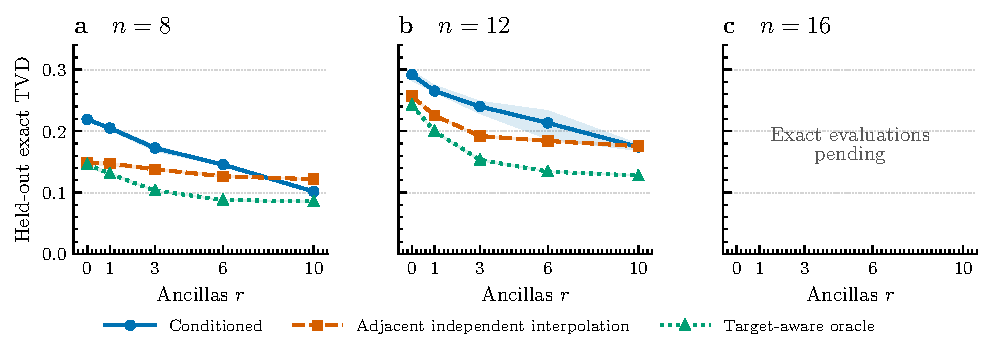
\includegraphics[width=\textwidth]{figures/gaussian_results.pdf}
\widefigurecaption{Held-out exact raw bitstring TVD for the Gaussian family as a function of the ancilla count at $n=8$ (left) and $n=12$ (right). Curves show medians over ten seeds after averaging the eight held-out conditions within each seed; shaded bands show the corresponding seed interquartile ranges. The conditioned model uses one shared circuit, independent interpolation combines neighboring independently trained models, and the target-aware oracle is fitted directly at each held-out condition. Lower values are better.}{fig:gaussian_results}
\end{minipage}
\end{plainwidetext}

The comparison with independent interpolation is more selective. At $n=8$, the independent bank is more accurate for $r\leq6$, but the shared model is better at $r=10$, with median TVD $0.102$ versus $0.122$. Its paired median advantage is $0.0198$ with interval $[0.0173,0.0211]$ and is positive in all ten seeds. At $n=12$ and $r=10$, the corresponding medians are $0.174$ and $0.175$; the paired advantage of $0.0049$ has interval $[-0.0077,0.0137]$, so the experiment does not resolve an advantage at this size. The direct target-aware fits reach $0.085$ and $0.128$ at eight and twelve qubits, leaving paired median oracle gaps of $0.016$ and $0.046$.

Additional midpoint probes illustrate the difference between evaluating a shared circuit and mixing neighboring output distributions. Figure~\ref{fig:gaussian-profiles} compares the $r=10$ models at $c\in\{0.125,0.375,0.875\}$, halfway between adjacent training conditions; the complementary $n=12$ profiles are in Appendix~\ref{app:qualitative-profiles}. The shared profiles follow the translated target peaks, whereas the independent mixtures are broader or displaced at these probes. We evaluate these conditions only after training and checkpoint selection; they supplement, rather than replace, the eight-condition held-out comparison. Their profile-level agreement does not imply an advantage in raw bitstring TVD across the full condition range.

\begin{plainwidetext}
\noindent\begin{minipage}{\textwidth}
\centering
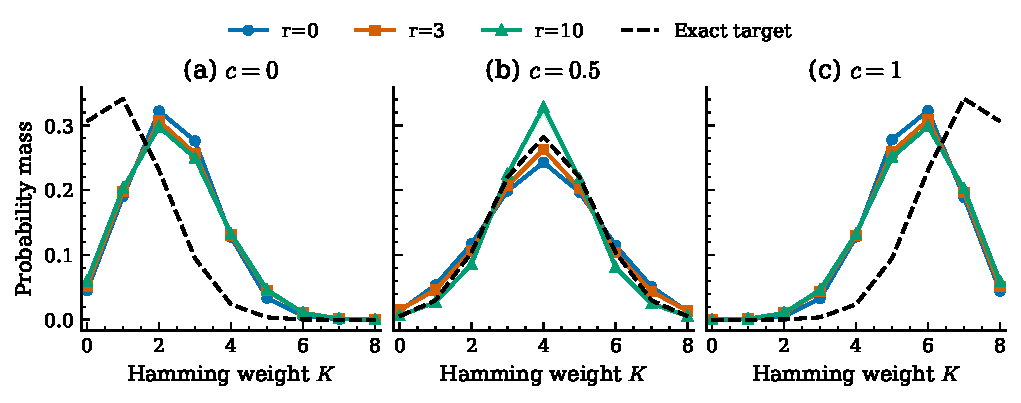
\includegraphics[width=\textwidth]{figures/gaussian_n8_training_profiles.pdf}
\medskip
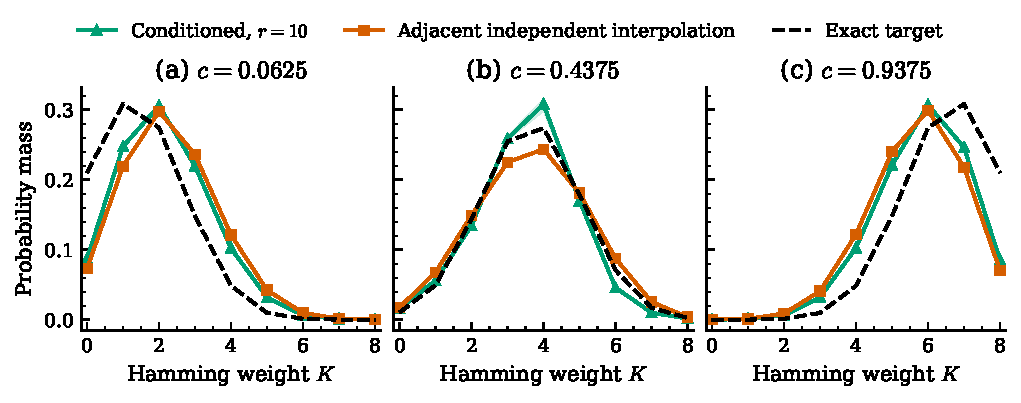
\includegraphics[width=\textwidth]{figures/gaussian_n8_generalization_profiles.pdf}
\widefigurecaption{Gaussian distribution shape at $n=8$. Top: reconstruction at training conditions $c\in\{0,0.5,1\}$ for $r\in\{0,3,10\}$; the endpoint displacement is already a reconstruction error. Bottom: shared $r=10$ predictions and adjacent-independent output interpolation at post-training midpoint probes $c\in\{0.125,0.375,0.875\}$. Probes did not enter training, validation or checkpoint selection. Curves show medians of exact Hamming-weight probabilities over ten seeds, bands show interquartile ranges, and dashed black curves are exact targets. Profile agreement need not imply low raw bitstring TVD.}{fig:gaussian-profiles}
\label{fig:app-gaussian-training-n8}\label{fig:app-gaussian-generalization-n8}
\end{minipage}
\end{plainwidetext}

The condition-resolved errors identify the main remaining limitation (Fig.~\ref{fig:app-gaussian-condition-response}). At $n=8$ and $r=10$, the shared median TVDs at the near-boundary held-out conditions $c=0.0625$ and $c=0.9375$ are $0.184$ and $0.188$, compared with $0.060$--$0.086$ at the six interior held-out conditions. Independent interpolation also degrades near the boundaries, while direct target-aware fits reach approximately $0.065$ there. The twelve-qubit results retain near-boundary errors and additional error around the centre. Thus, the shared circuit follows the translated family with improved accuracy as ancillas increase, but neither the profiles nor the raw-TVD results support uniformly accurate interpolation. The present comparison does not isolate whether the remaining error comes from the condition map, parameter sharing, or optimization.



\subsection{Curie--Weiss temperature response}

Curie--Weiss requires the model to change the shape of the distribution, from a central magnetization peak to two ordered modes. The profiles at $\beta\in\{0.6,1,1.4\}$ show this response at eight and twelve qubits (Fig.~\ref{fig:curie-profiles}; complementary $n=8$ profiles appear in Appendix~\ref{app:qualitative-profiles}). Without ancillas, the shared model exhibits pronounced shell-to-shell oscillations in the disordered and crossover regimes. Adding ancillas suppresses these oscillations and improves the allocation of probability across magnetization shells. At $n=12$ and $\beta=1.4$, however, the $r=10$ model still misallocates mass near the edges and centre despite retaining a two-mode profile. The improvement therefore concerns distribution shape as well as the average error, but does not amount to exact reconstruction.

The raw bitstring TVD confirms the improvement visible in the profiles (Fig.~\ref{fig:curie-production-results}). Averaging all five held-out temperatures within each seed, the median decreases from $0.190$ to $0.047$ between $r=0$ and $r=10$ at $n=8$, and from $0.275$ to $0.076$ at $n=12$. The median decreases at each tested ancilla count for both sizes. The paired median changes are $-0.143$ with 95\% bootstrap interval $[-0.148,-0.142]$ and $-0.198$ with interval $[-0.202,-0.193]$, respectively. These are aggregate improvements, not monotonicity guarantees for every condition or fit.

\begin{plainwidetext}
\noindent\begin{minipage}{\textwidth}
\centering
    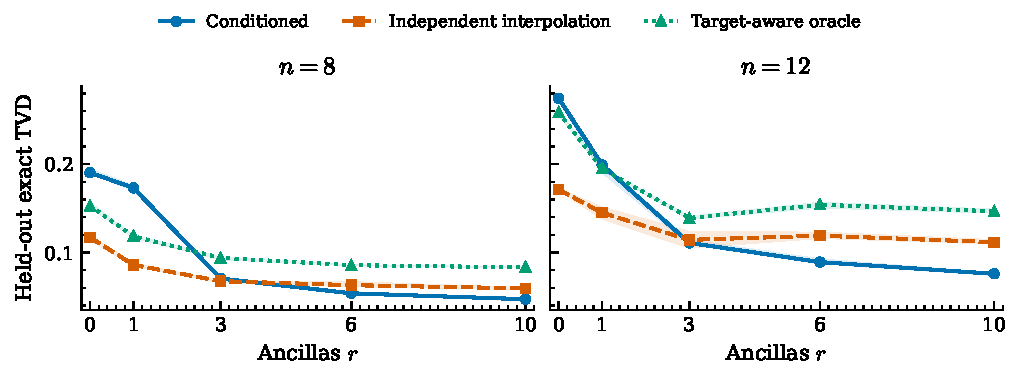
\includegraphics[width=\textwidth]{figures/curie_weiss_results.pdf}
    \widefigurecaption{Ancilla scaling of held-out exact raw bitstring TVD for the Curie--Weiss production campaign at $n=8$ (left) and $n=12$ (right). Curves show medians and bands show interquartile ranges over ten seeds after averaging all five held-out temperatures within each seed. This average includes the prescribed $\beta=1$ landmark; the text reports non-landmark interpolation separately. The target-aware oracle denotes direct independent fits under the fixed training protocol, not globally optimal circuits.}{fig:curie-production-results}
\end{minipage}
\end{plainwidetext}

The advantage persists when the supplied $\beta=1$ landmark is excluded. At $r=10$, averaging only $\beta\in\{0.6,0.8,1.2,1.4\}$ gives median conditioned TVDs of $0.047$ and $0.081$ for $n=8$ and $n=12$, respectively, compared with $0.058$ and $0.117$ for adjacent-independent interpolation. The paired median advantages are $0.0119$ with interval $[0.0080,0.0136]$ and $0.0363$ with interval $[0.0299,0.0433]$; both are positive in every matched seed. The improvement concerns interpolation within the prescribed, problem-informed temperature map, not discovery of the transition location.

At the prescribed landmark itself, the $r=10$ conditioned model attains median exact TVDs of $0.048$ and $0.054$ for $n=8$ and $n=12$. Averaging the three-point window $\beta\in\{0.8,1,1.2\}$ gives $0.057$ and $0.079$. The condition-resolved curves in Fig.~\ref{fig:app-curie-condition-response} place these values within the full temperature response. Both the shared model and independent interpolation reproduce the broad change in magnetization shape (Fig.~\ref{fig:curie-profiles}, lower panels; Fig.~\ref{fig:app-curie-generalization} gives the $n=8$ check), so the quantitative comparison is necessary to distinguish them. In particular, a close profile can hide within-shell error: at $n=12$ and $r=10$, the full held-out profile-TVD median is $0.063$, below the raw bitstring value $0.076$.

The direct target-aware fits do not provide a lower bound on achieved error. At $r=10$, their median non-landmark TVDs are $0.084$ and $0.152$, exceeding the conditioned values at both sizes. A shared fit receives data from six training temperatures, whereas each independent fit receives data from one temperature, and both use a finite optimization budget. The observed ordering therefore compares the implemented training procedures; it does not show that a shared circuit has greater single-condition capacity. Conversely, at low ancilla counts, interpolation between independent outputs remains more accurate than the shared model. The benefit of sharing depends on the ancilla count and the benchmark.

\begin{plainwidetext}
\noindent\begin{minipage}{\textwidth}
\centering
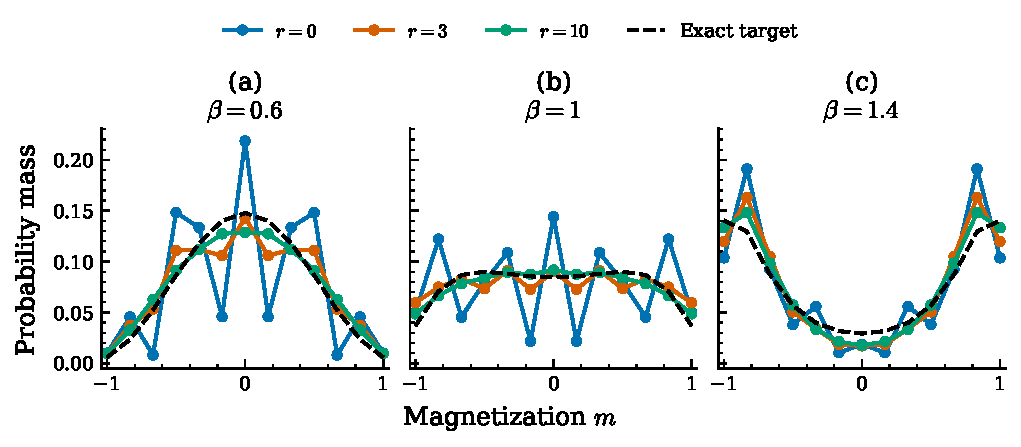
\includegraphics[width=\textwidth]{figures/curie_weiss_n12_magnetization_profiles.pdf}
\medskip
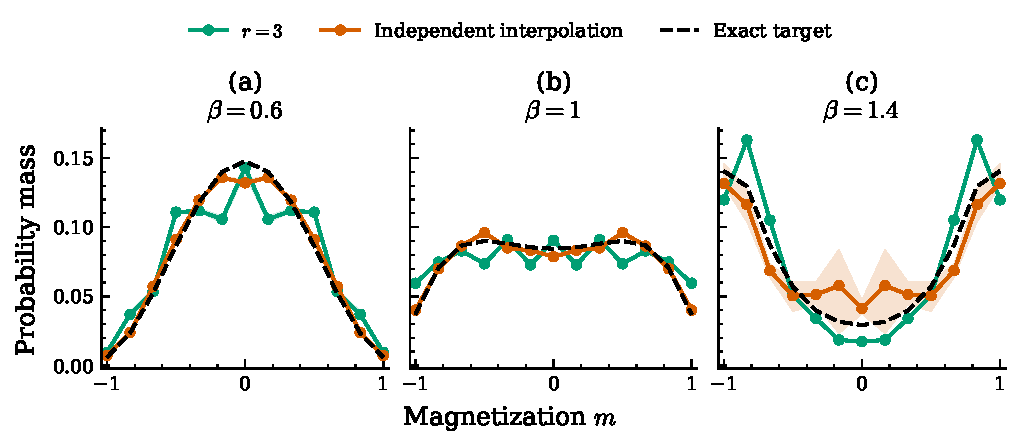
\includegraphics[width=\textwidth]{figures/curie_weiss_n12_generalization_profiles.pdf}
\widefigurecaption{Curie--Weiss distribution shape at $n=12$ and held-out $\beta\in\{0.6,1,1.4\}$. Top: increasing the ancilla count suppresses shell oscillations, while ordered-regime residuals remain. Bottom: the shared $r=10$ model and interpolation between neighboring independent outputs both reproduce the broad shape change. Curves show medians of exact magnetization probabilities over ten seeds, bands show interquartile ranges, and dashed black curves are exact targets. The $\beta=1$ panel tests the prescribed landmark, not discovery of its location; raw bitstring TVD also measures errors hidden within magnetization shells.}{fig:curie-profiles}
\label{fig:app-curie-profiles-n12}\label{fig:app-curie-generalization-n12}
\end{minipage}
\clearpage
\end{plainwidetext}

\subsection{Curie--Weiss conditioning ablation}
\label{sec:curie-ablation}

The production results combine a spin-flip-symmetric input, a problem-informed condition map, and ancillas. To separate their contributions, the eight-qubit ablation crosses product and spin-flip inputs with affine and informed maps, at $r\in\{0,10\}$ and three matched seeds. Figure~\ref{fig:curie-weiss} shows the product--affine and spin-flip--informed combinations; the comparisons below also include the two crossed combinations. This smaller study tests which design choices account for the temperature response, rather than extending the ten-seed production comparison.

\begin{center}
\begin{minipage}{\columnwidth}
\centering
    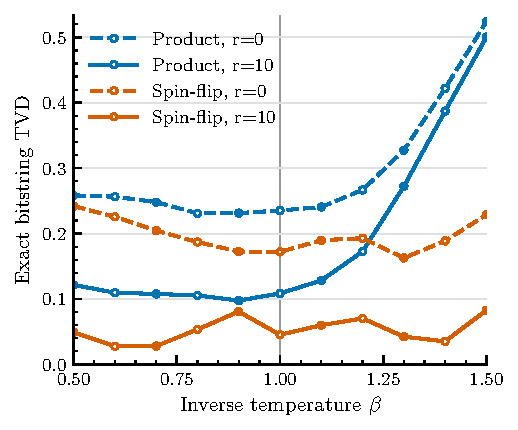
\includegraphics[width=\columnwidth]{figures/curie_encoder_ablation_n8.pdf}
    \widefigurecaption{Exact bitstring TVD across inverse temperature for the $n=8$ Curie--Weiss ablation. The product input uses the generic affine map, whereas the spin-flip input uses the informed piecewise-linear map. Curves show medians over three matched seeds. Filled markers denote training temperatures and open markers denote held-out temperatures; line style distinguishes $r=0$ from $r=10$. The vertical line marks $\beta=1$, which is a prescribed landmark only for the informed map. Lower values are better.}{fig:curie-weiss}
\end{minipage}
\end{center}

Ancillas improve all four encoder--map combinations in each of the three matched seeds. For the product input with the affine map, the median exact TVD over the four non-landmark held-out temperatures decreases from $0.295$ at $r=0$ to $0.194$ at $r=10$; at $\beta=1$, it decreases from $0.235$ to $0.108$. Because this map has no feature at $\beta=1$, the improvement does not require a supplied transition landmark.

The generic product construction nevertheless failed to reproduce the ordered magnetization profile. For $r=10$ and $\beta\in\{1.2,1.3,1.4\}$, its median Hamming-weight profile placed the two modes near weights $2$ and $6$, whereas the target modes lie at weights $0$ and $8$ for $n=8$. At $\beta=1.5$, the learned profile no longer retained the target's two-mode structure. The informed spin-flip construction with $r=10$ preserved the symmetric modes at weights $0$ and $8$ throughout this ordered range. Ancillas therefore improved the generic product model without fully recovering the target bimodality.

Problem-informed conditioning attained comparable non-landmark error with fewer qubits in this development screen. The spin-flip input with the informed map attained a median non-landmark TVD of $0.193$ without ancillas, close to the $0.194$ attained by the generic product construction with ten ancillas. These circuits store 36 and 171 phase coordinates, respectively; 55 coordinates in the latter act only on ancillas, leaving at most 116 visible-affecting directions. Input-preparation costs are not matched by this count. This comparison does not imply that symmetry alone substitutes for ancillas. With the generic map, replacing the product input by the spin-flip input changed the non-landmark TVD from $0.295$ to $0.308$ at $r=0$ and from $0.194$ to $0.198$ at $r=10$. The informed map improved both input families, and the spin-flip input became useful when paired with it: at $r=10$, the median non-landmark TVD decreased from $0.115$ for the informed product input to $0.047$ for the informed spin-flip input. The latter construction also attained $0.045$ at $\beta=1$ and remained below $0.083$ at every evaluated temperature.

Table~\ref{tab:curie-ablation-complete} summarizes all four combinations. The ablation therefore suggests encoder--map dependence; differences of three-seed medians are descriptive and do not constitute a confirmatory paired interaction test. Symmetry alone does not improve the reported non-landmark average under the affine map, whereas the spin-flip input with the informed map gives the lowest error among the tested combinations. Ancillas improve both product and spin-flip constructions, but do not fully compensate for the product--affine encoder's failure to reproduce the ordered modes. These conclusions concern the tested maps and three development seeds; the ten-seed campaign supplies the main accuracy and interpolation estimates.

\begin{center}
\begin{minipage}{\columnwidth}
\refstepcounter{table}\label{tab:curie-ablation-complete}
\small
Table~\thetable: Curie--Weiss ablation at $n=8$. Median raw TVD over three seeds after averaging the four non-landmark held-out temperatures; all encoder--map combinations are shown.
\par\vspace{5pt}\centering
\begin{tabular}{@{}lrr@{}}
\toprule
Input / map & $r=0$ & $r=10$ \\
\midrule
Product / affine & .2947 & .1941 \\
Spin-flip / affine & .3084 & .1981 \\
Product / informed & .2190 & .1154 \\
Spin-flip / informed & .1935 & .0466 \\
\bottomrule
\end{tabular}
\end{minipage}
\end{center}


\subsection{Spatial generation with two conditional inputs}
\label{sec:at-results}

The Ashkin--Teller experiment tests whether the reference interface extends to spatially structured inputs and new combinations of known couplings. Figure~\ref{fig:at-summary} compares all six models at both sizes. Mean held-out TVD is $0.1327$ for symmetry-only IQP and $0.0933$ for bond-informed IQP at $n=8$; at $n=12$ the corresponding values are $0.2737$ and $0.1893$. The paired bond-minus-cat differences are $-0.0395$ with interval $[-0.0418,-0.0370]$ and $-0.0844$ with interval $[-0.0892,-0.0802]$. These comparisons favor the bond-informed family under the matched circuit and training budgets within each size.

\begin{plainwidetext}
\noindent\begin{minipage}{\textwidth}
\centering
 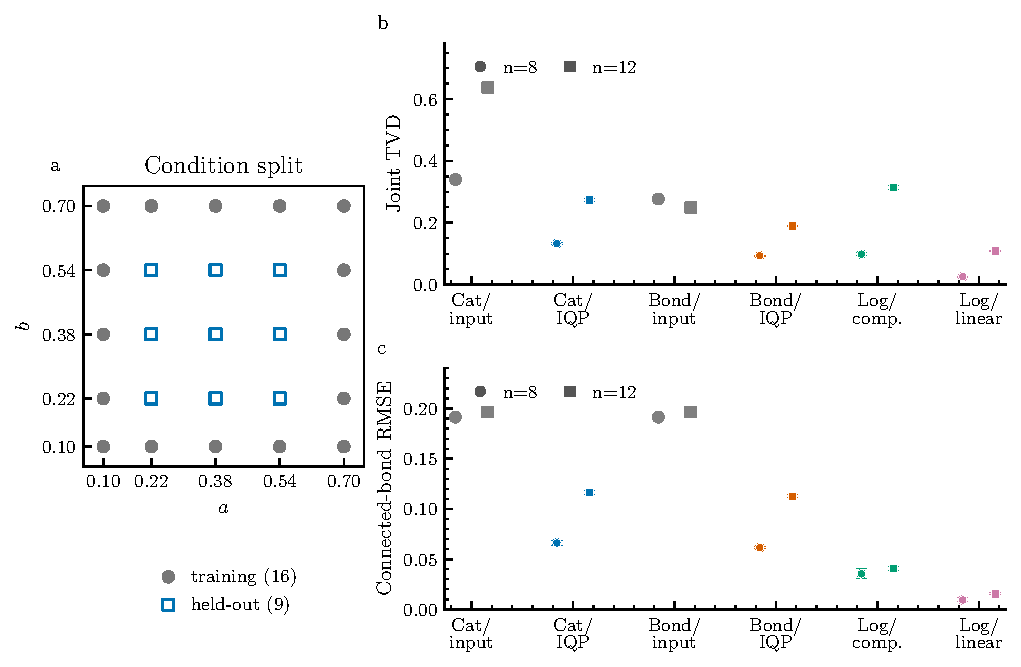
\includegraphics[width=\textwidth]{figures/ashkin_teller_paper_summary.pdf}
 \widefigurecaption{Conditional generation on two coupled periodic rings. (a) Perimeter training conditions and held-out interior combinations. (b,c) Exact held-out joint TVD and connected-bond correlation RMSE. Circles denote $n=8$ and squares $n=12$, with parameters trained separately at each size. Points average nine conditions within each seed and then ten seeds; error bars are percentile 95\% bootstrap intervals over seeds and may be smaller than the markers. Grey inputs are deterministic controls. Cat and bond denote symmetry-only and bond-informed inputs. Classical predictors share the sampled training and validation data but use different parameterizations.}{fig:at-summary}
\end{minipage}
\end{plainwidetext}

Both shared circuits improve joint TVD and connected-bond error over their own input in every one of the 90 seed/condition pairs at each size. At $n=12$, the symmetry-only and bond input TVDs are $0.6385$ and $0.2500$, respectively. The bond input therefore contributes substantial prior structure, but the learned circuit still reduces its joint error and supplies useful interlayer dependence. The comparison changes the complete encoder family, including its input phases and coupling response; it does not isolate a topology-only effect.

Figure~\ref{fig:at-structure} tests arrangement beyond each output's joint layer-weight profile and dependence beyond its full layer marginals; Appendix~\ref{app:at-diagnostics} specifies the transformations. Removing either increases TVD for both quantum models in all 90 pairs at $n=8$. At $n=12$, spatial arrangement remains helpful in every pair, while dependence is helpful in all bond-informed outputs but detrimental in 13 symmetry-only pairs. Lower joint TVD does not imply uniformly better correlation recovery: bond-informed IQP has higher condition-mean connected-bond error than symmetry-only IQP at one condition for $n=8$ and four for $n=12$. At $n=12$, their mean correlation RMSEs are $0.1127$ and $0.1162$, with worst condition means $0.1938$ and $0.1867$. Some bond-output marginal errors also worsen relative to its input despite improved joint TVD.

The pooled classical log-linear predictor is more accurate than both IQP models, with TVD $0.0260$ at $n=8$ and $0.1088$ at $n=12$. Its affine conditional log odds are well specified for Eq.~\eqref{eq:at-target}. Empirical log composition yields $0.0988$ and $0.3145$. These baselines provide classical context for a methods demonstration, not evidence of quantum advantage. Both trained quantum errors rise at the larger size under the fixed sampling and update budgets; the larger encoder-family gap does not establish favorable scaling. Full condition-level TVD and correlation results are retained in Tables~\ref{tab:at-conditions-n8} and~\ref{tab:at-conditions-n12}.

\begin{plainwidetext}
\noindent\begin{minipage}{\textwidth}
 \centering
 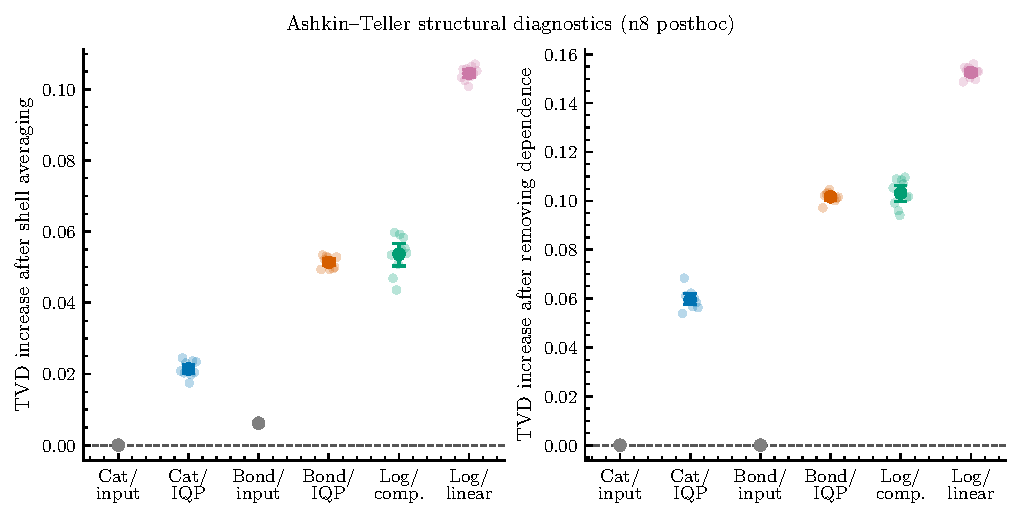
\includegraphics[width=\textwidth]{figures/ashkin_teller_structure_n8.pdf}
 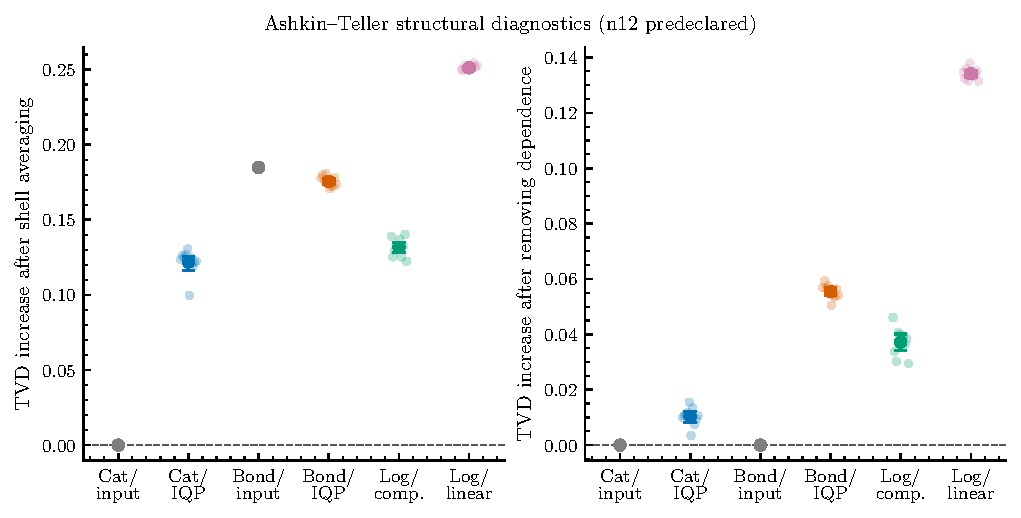
\includegraphics[width=\textwidth]{figures/ashkin_teller_structure_n12.pdf}
 \widefigurecaption{Spatial and dependence diagnostics for all six models at $n=8$ (top, post hoc) and $n=12$ (bottom, predeclared). Faint points show seed means, solid points show the mean and bars show percentile 95\% bootstrap intervals. Grey encoder-only controls are deterministic. Left: TVD change after redistributing mass uniformly within each joint layer-weight shell. Right: TVD change after replacing the joint output by the product of its full layer marginals. Positive values mean the original output is closer to the target than its transformed distribution; these changes do not measure improvement over the input. The transformations are defined in Appendix~\ref{app:at-diagnostics}. Seed means can be positive while individual condition deltas are negative; all condition results are retained in the accompanying artifacts.}{fig:at-structure}
\end{minipage}
\end{plainwidetext}


\subsection{Training data and ancilla capacity}
\label{sec:data-ancilla-results}

Figure~\ref{fig:data-ancilla} reports the crossed follow-up. Increasing training examples per condition from 100 to 1,000 reduces mean interior TVD in every learned arm. Symmetry-only IQP changes from $0.2981$ to $0.2774$ without ancillas and from $0.2778$ to $0.2659$ with four. Bond-informed IQP changes from $0.2256$ to $0.1920$ without ancillas and from $0.2244$ to $0.1920$ with four. Much of the quantum improvement occurs by 300 examples. The symmetry-only zero-ancilla mean then rises from $0.2725$ to $0.2774$, showing a nonmonotonic response under the fixed update budget.

\begin{plainwidetext}
\noindent\begin{minipage}{\textwidth}
\centering
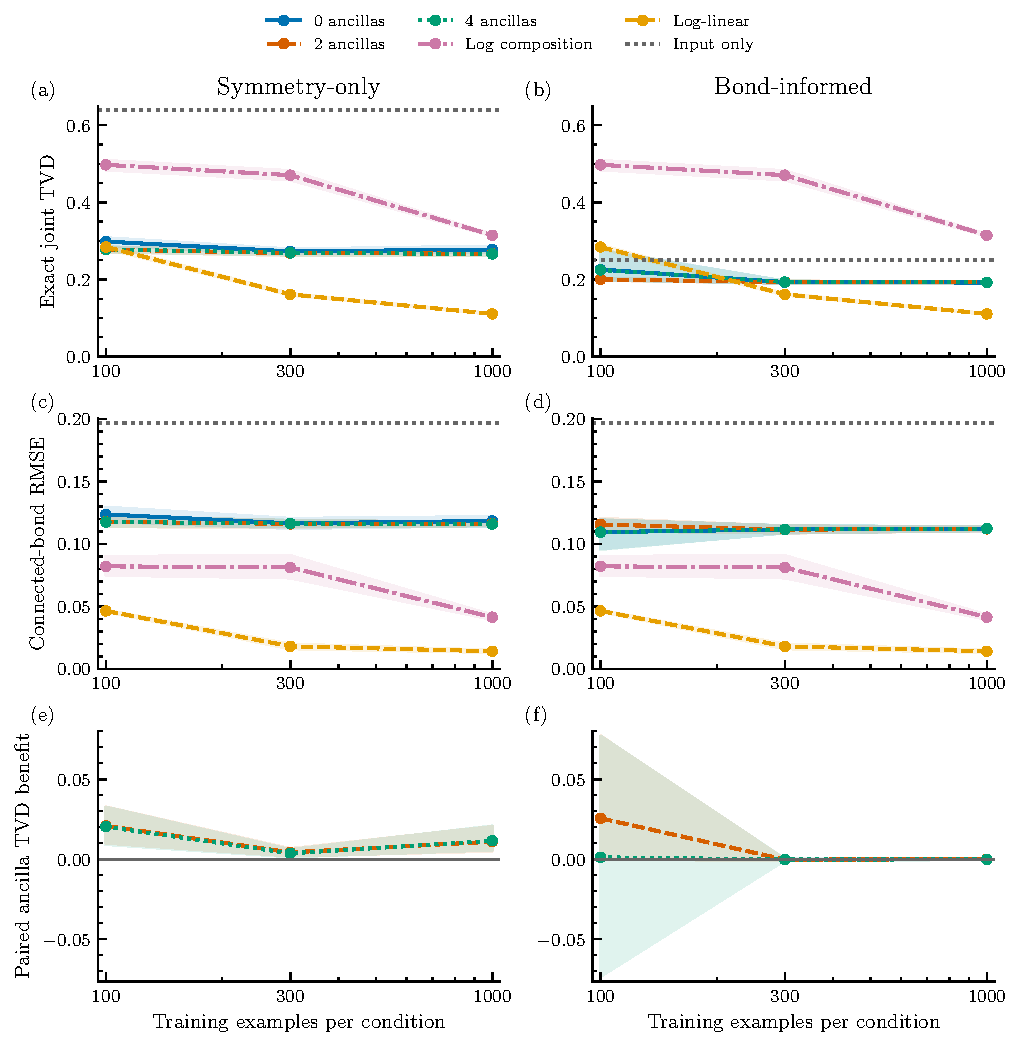
\includegraphics[width=0.97\textwidth]{figures/data_ancilla_learning_curves.pdf}
\widefigurecaption{Training-data sensitivity and ancilla effects at twelve visible qubits. Columns compare symmetry-only and bond-informed encodings. (a,b) Exact joint TVD; (c,d) connected-bond correlation RMSE; (e,f) paired TVD benefit $E_{s,0}-E_{s,r}$ for two and four ancillas, where positive values favor ancillas. Points average nine interior conditions within each seed and then ten fresh paired seeds; shaded regions are descriptive percentile 95\% intervals from 10,000 paired seed resamples. Lines connect the three measured training sizes on a logarithmic axis. Classical predictors are fitted once per seed and size and repeated in both columns for comparison; grey input controls are deterministic. Each fit additionally accesses 1,000 independent validation examples per condition (16,000 in total), and each IQP fit receives 500 updates. Thus the horizontal axis measures training examples, not total labeled access. Active phase counts are 78, 102 and 126 for zero, two and four ancillas.}{fig:data-ancilla}
\end{minipage}
\end{plainwidetext}

The paired four-ancilla TVD benefits for symmetry-only IQP are $0.0203$, $0.0037$ and $0.0115$ at the three data sizes. Its primary interaction is $-0.0088$ with interval $[-0.0219,0.0032]$; the bond-informed interaction is $-0.0012$ with interval $[-0.0768,0.0731]$. Neither establishes a growing benefit with training data, nor equivalence or absence of interaction. The two-ancilla interaction intervals also include zero. At 300 and 1,000 examples, bond-informed TVD means differ by less than $0.0003$ across ancilla counts. At 100 examples, isolated zero- and four-ancilla fits have TVD $0.4505$ and $0.4436$, in different seeds; remaining fits in those arms range from $0.1934$ to $0.2072$. Both poor fits are retained, producing substantial paired uncertainty.

The pooled log-linear predictor improves from $0.2840$ to $0.1611$ to $0.1105$, outperforming every quantum arm in joint TVD at 300 and 1,000 examples. Log composition improves from $0.4971$ to $0.4702$ to $0.3145$. Log-linear connected-bond RMSE falls from $0.0464$ to $0.0141$, while quantum means remain between $0.1094$ and $0.1236$. All quantum mean joint and connected-bond errors improve over their input controls; the poor fits prevent an every-seed claim. Complete paired contrasts, marginal errors and worst-condition diagnostics accompany the result artifacts.

\subsection{Scope of the interpolation results}

Across the four Gaussian and Curie--Weiss dataset--size combinations, increasing the ancilla count reduces median held-out raw TVD, but it does not uniformly make sharing preferable to independent interpolation. The clearest interpolation advantages occur for the ten-ancilla Gaussian model at eight qubits and for the ten-ancilla Curie--Weiss model at both sizes, including the non-landmark temperatures. Gaussian interpolation at twelve qubits remains statistically unresolved against the independent bank. Figure~\ref{fig:app-training-heldout-scaling} compares reconstruction and held-out error along the same ancilla ladders. The held-out-minus-training gap is descriptive rather than a matched-condition test: the two averages cover different conditions, and the training sets include the endpoints where reconstruction can be difficult. A negative gap therefore does not establish that unseen conditions are intrinsically easier to learn. Together, the results support within-range conditional generation with an ancilla-dependent accuracy benefit, while leaving the boundary response and the contribution of problem-specific encoding as explicit limitations.

\section{Discussion}
The experiments address two aspects of the conditional construction. Gaussian and Curie--Weiss targets measure the accuracy cost of sharing and the combined effect of ancilla capacity and conditioning. Ashkin--Teller tests a spatial two-input family and correlated reference access. The latter extends the demonstrated input constructions beyond Hamming-shell amplitudes, while retaining the same phase-gradient estimator. Sampled-MMD checkpoint selection in that study also separates fitting from exact final evaluation.

Prior information remains central to interpretation. The Curie--Weiss encoder uses a prescribed temperature map; the bond encoder supplies the uncoupled ring law, its topology and coupling dependence. Encoder-only controls establish an additional learned contribution on Ashkin--Teller, but neither comparison establishes a causal benefit from symmetry or topology alone. The classical log-linear result demonstrates that this benchmark has a suitable classical conditional representation. The target's tractability is compatible with evaluating the proposed interface, but limits claims about competitive modeling of unknown distributions.

The crossed study distinguishes encoder and ancilla effects: symmetry-only IQP gains modestly from ancillas, whereas bond-informed mean TVD is nearly unchanged across ancilla counts at 300 and 1,000 training examples. The primary interaction remains unresolved for both encoders. Fixed validation access supplies a common selection resource, but the additional 16,000 validation examples preclude a few-label claim. Fixed updates change the number of data passes, and the growing phase count prevents attribution solely to latent capacity. These results characterize this training procedure, without identifying optimal sample complexity or a universal ancilla requirement.

All held-out evidence concerns interpolation within the prescribed domains. Earlier exploratory Ashkin--Teller joint-extrapolation tests failed to establish reliable generalization; the present perimeter/interior split does not resolve that limitation. The dependence and marginal exceptions further show why joint TVD and selected observables must be reported separately. Neither two trained sizes nor efficient reference access establishes asymptotic trainability, efficient classical output sampling or a quantum hardware advantage. State-preparation precision, routing and exact evaluation costs remain separate from the arithmetic cost of the training estimator.

\section{Conclusions}
We formulate conditional IQP generation with one fixed learned diagonal unitary and a condition-dependent input supporting classical sampling and amplitude-ratio evaluation. Product, cat-like and correlated ring constructions realize this interface. Experiments demonstrate within-range conditional response, ancilla-dependent accuracy improvements on Gaussian and Curie--Weiss targets, and two-input spatial interpolation with Ashkin--Teller inputs. The results also expose sharing costs, sensitivity to supplied input structure and incomplete dependence recovery. They support the conditional construction within these tested settings, without establishing quantum advantage or general extrapolation.

\clearpage
\appendix
\section{Representative exact distribution profiles}
\label{app:qualitative-profiles}

This appendix provides condition-resolved checks and complementary-size profiles for the main-text examples in Figs.~\ref{fig:gaussian-profiles} and~\ref{fig:curie-profiles}. It distinguishes reconstruction at training conditions from interpolation to untrained conditions. We fixed three conditions in each comparison by scientific role rather than fit quality. Each learned curve shows the median exact visible distribution over ten production seeds, and the shaded region shows the corresponding interquartile range. These profiles supplement the exact-TVD summaries by showing which parts of each distribution the models reproduce or miss.

\subsection{Ancilla scaling and condition-resolved errors}

\begin{plainwidetext}
\noindent\begin{minipage}{\textwidth}
    \centering
    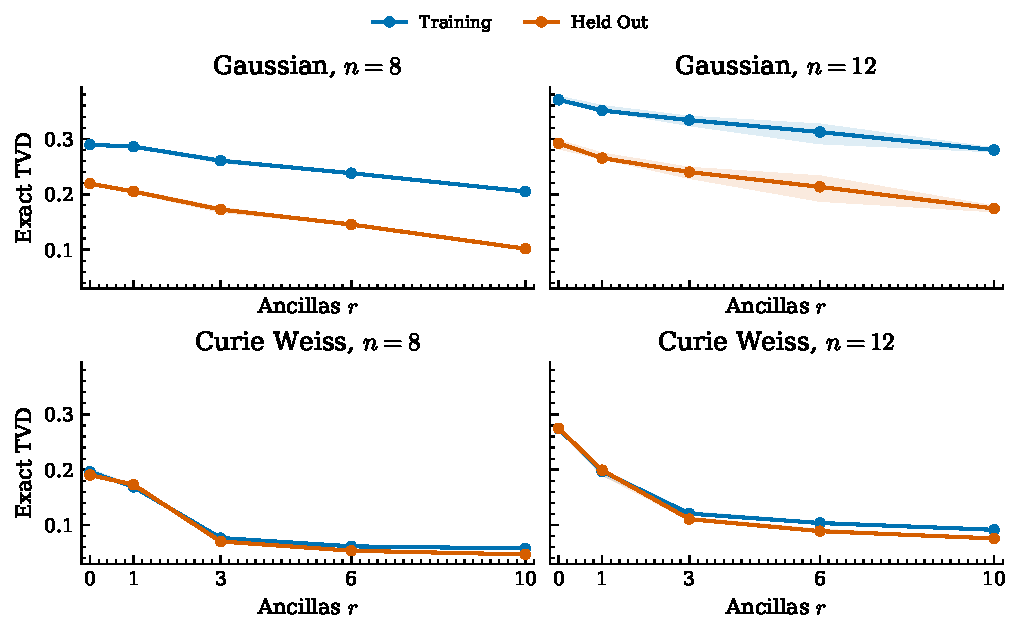
\includegraphics[width=\textwidth]{figures/conditioned_training_vs_heldout.pdf}
    \widefigurecaption{Exact raw bitstring TVD of the conditioned model at training and held-out conditions for all four dataset--size combinations. Curves show medians and bands show interquartile ranges after averaging the corresponding condition set within each seed. A negative held-out-minus-training gap does not imply better generalization than reconstruction: the two averages use different conditions, and the training sets include the domain endpoints. The Curie--Weiss held-out average includes the supplied $\beta=1$ landmark.}{fig:app-training-heldout-scaling}
\end{minipage}
\end{plainwidetext}

\begin{plainwidetext}
\noindent\begin{minipage}{\textwidth}
    \centering
    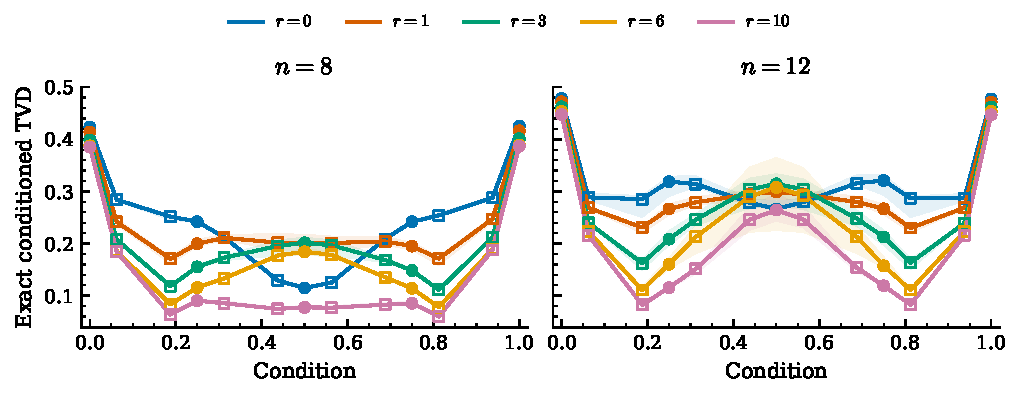
\includegraphics[width=\textwidth]{figures/gaussian_condition_response.pdf}
    \widefigurecaption{Condition-resolved exact raw TVD for the Gaussian model at $n=8$ and $n=12$ across all five ancilla counts. Curves show medians and bands show interquartile ranges over ten seeds at each condition. Filled markers denote training conditions and open markers denote held-out conditions. Endpoint errors persist despite the improvement with ancillas; these are reconstruction errors at training conditions rather than evidence of extrapolation failure.}{fig:app-gaussian-condition-response}
    \medskip
    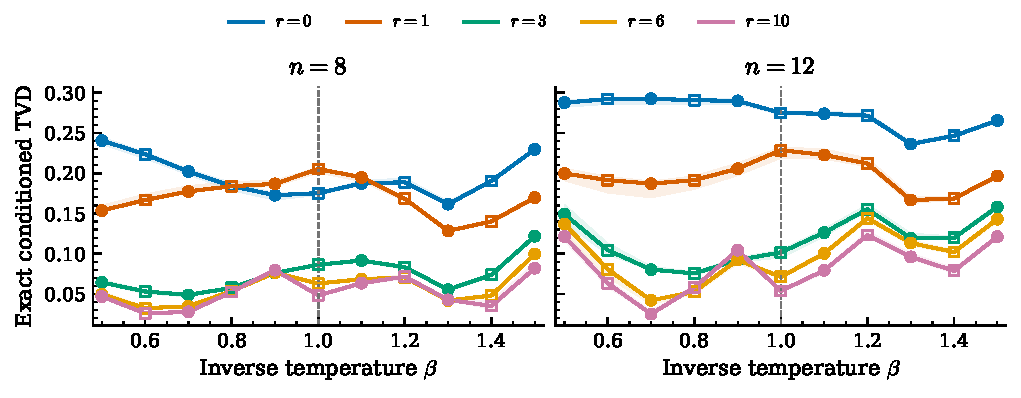
\includegraphics[width=\textwidth]{figures/curie_weiss_condition_response.pdf}
    \widefigurecaption{Condition-resolved exact raw TVD for the Curie--Weiss model at $n=8$ and $n=12$. Marker and uncertainty conventions follow Fig.~\ref{fig:app-gaussian-condition-response}. The vertical line marks the supplied $\beta=1$ landmark. The full condition response complements the averaged ancilla ladder and exposes residual errors away from the landmark.}{fig:app-curie-condition-response}
\end{minipage}
\end{plainwidetext}

\clearpage

\begin{plainwidetext}
\noindent\begin{minipage}{\textwidth}
\subsection{Complementary Gaussian profiles}
    \centering
    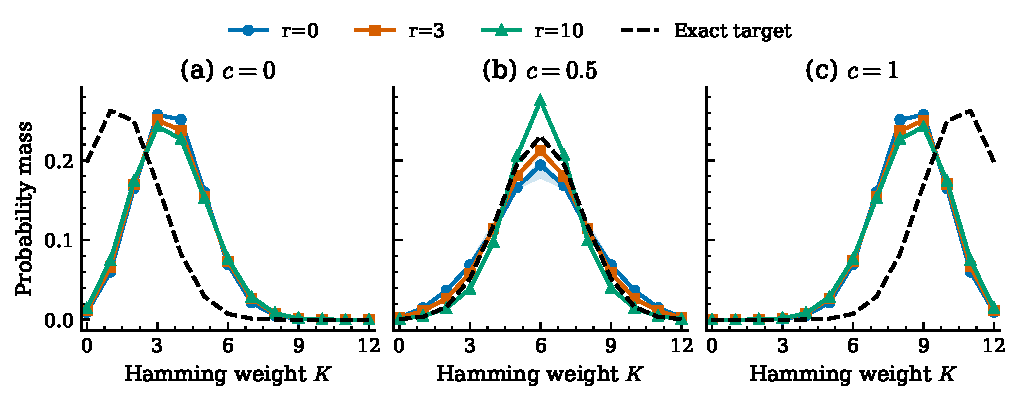
\includegraphics[width=\textwidth]{figures/gaussian_n12_training_profiles.pdf}
    \widefigurecaption{Gaussian Hamming-weight profiles at the training conditions $c\in\{0,0.5,1\}$ for $n=12$. Curves and uncertainty summaries follow the upper panels of Fig.~\ref{fig:gaussian-profiles}. The endpoint modes remain displaced towards the centre of the Hamming-weight range, whereas the model reproduces the central target more accurately.}{fig:app-gaussian-training-n12}
\end{minipage}
\end{plainwidetext}


\begin{plainwidetext}
\noindent\begin{minipage}{\textwidth}
    \centering
    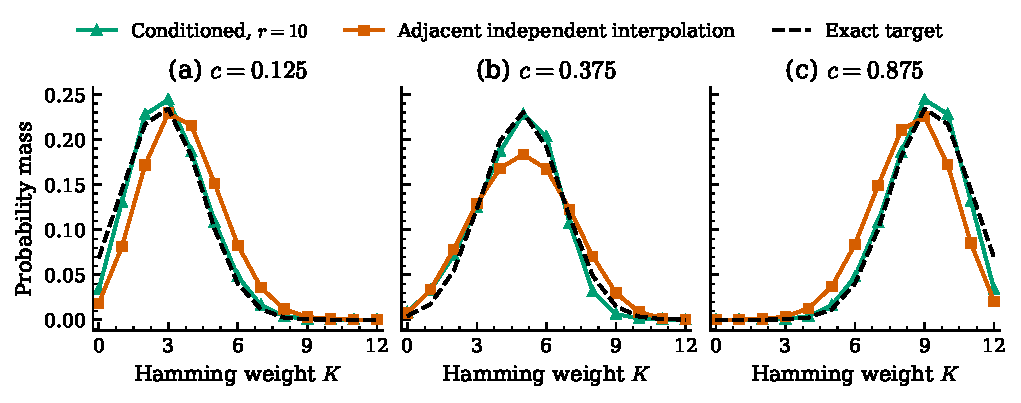
\includegraphics[width=\textwidth]{figures/gaussian_n12_generalization_profiles.pdf}
    \widefigurecaption{Gaussian Hamming-weight profiles at the post-training midpoint probes $c\in\{0.125,0.375,0.875\}$ for $n=12$. The probe construction, interpolation rule, and uncertainty summaries follow the lower panels of Fig.~\ref{fig:gaussian-profiles}. The conditioned model again tracks the exact target across the three probes, whereas interpolation between independent models produces broader or displaced profiles.}{fig:app-gaussian-generalization-n12}
\end{minipage}
\end{plainwidetext}

\clearpage
\begin{plainwidetext}
\noindent\begin{minipage}{\textwidth}
\subsection{Complementary Curie--Weiss profiles}
    \centering
    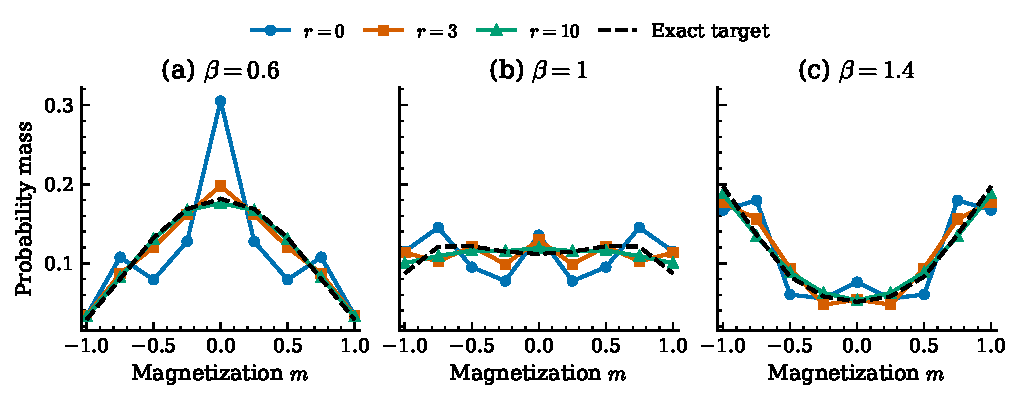
\includegraphics[width=\textwidth]{figures/curie_weiss_n8_magnetization_profiles.pdf}
    \widefigurecaption{Representative Curie--Weiss magnetization profiles for $n=8$ in the disordered regime at $\beta=0.6$ (a), at the prescribed transition landmark $\beta=1$ (b), and in the ordered regime at $\beta=1.4$ (c). Curves show medians over ten production seeds, and shaded bands show interquartile ranges. Increasing the ancilla count suppresses shell-to-shell oscillations in panels (a) and (b) and recovers the two edge modes in panel (c). Because the condition map contains the $\beta=1$ landmark, panel (b) tests reconstruction at the transition but not unbiased interpolation of its location.}{fig:app-curie-profiles}
\end{minipage}
\end{plainwidetext}

\begin{plainwidetext}
\noindent\begin{minipage}{\textwidth}
    \centering
    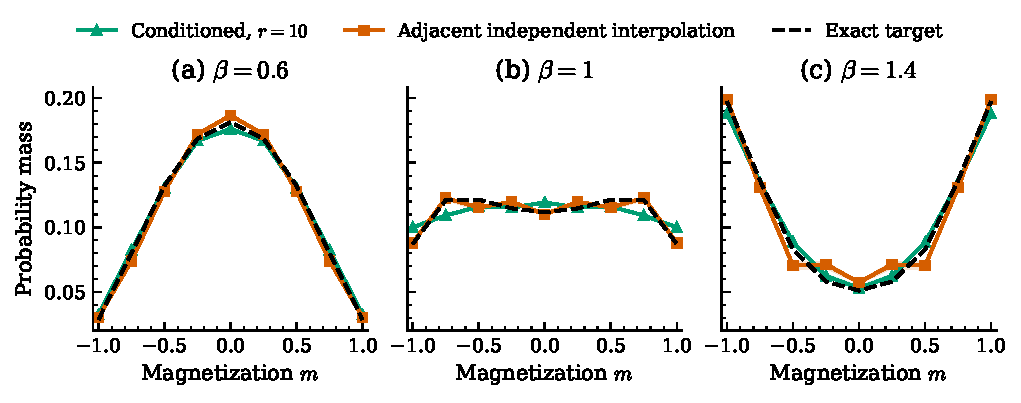
\includegraphics[width=\textwidth]{figures/curie_weiss_n8_generalization_profiles.pdf}
    \widefigurecaption{Curie--Weiss magnetization profiles at the held-out inverse temperatures $\beta\in\{0.6,1,1.4\}$ for $n=8$. The conditioned model directly evaluates each held-out temperature with $r=10$, whereas the adjacent-independent baseline linearly interpolates, separately within each seed, the exact output distributions of the two neighboring $r=10$ independent circuits. Curves show medians over ten production seeds, and shaded bands show interquartile ranges. Both approaches reproduce the change from the central disordered mode to the ordered edge modes. Because the informed condition map contains the $\beta=1$ landmark, the central panel tests reconstruction at that prescribed landmark rather than unbiased localization of the transition.}{fig:app-curie-generalization}
\end{minipage}
\end{plainwidetext}

\clearpage

\section{Correlated reference access and preparation}
\label{app:at-reference}

Expanding the trace in Eq.~\eqref{eq:bond-transfer-amplitude} over cyclic physical spins gives the Hadamard transform of Eq.~\eqref{eq:bond-input}. The $\mathbb Z_2$ symmetry makes $\psi_g(z)$ vanish at odd parity; the two-ring reference has even parity in each layer. We enforce these support zeros exactly. A ratio can have a zero numerator, but its denominator is queried only at a sampled nonzero-support state.

For sequential reference sampling, define $\mathcal E_z=A_z\otimes\overline{A_z}$ and $\mathcal S=\mathcal E_0+\mathcal E_1$. The probability of a length-$k$ prefix, apart from the common normalization $2^m Z_m(g)$, is
\begin{equation}
 w(z_0,\ldots,z_{k-1})=\operatorname{tr}\!\left[\mathcal E_{z_0}\cdots\mathcal E_{z_{k-1}}\mathcal S^{m-k}\right].
\end{equation}
Indeed, $|\operatorname{tr}M|^2=\operatorname{tr}(M\otimes\overline M)$, and summing over each unobserved bit replaces its doubled matrix by $\mathcal S$. The two child-prefix weights normalized by their sum give the next-bit probability. Precomputing the suffix powers takes $O(m)$ arithmetic and each draw uses $O(m)$ fixed-dimension contractions. The two rings are sampled independently. Amplitudes and their ratios use Eq.~\eqref{eq:bond-transfer-amplitude}, with the common normalization cancelling in the ratio.

This arithmetic bound assumes controlled numerical precision. Common positive rescaling stabilizes prefix and suffix contractions; it does not remove cancellation in very small amplitudes. The implementation rescales the amplitude transfer matrix by $2\cosh(g/2)$ in the ratio path. Enumeration checks cover reference probabilities, moments, phase gradients and both layer flips at the tested sizes, and separate tests verify coherent preparation amplitudes. These checks do not establish uniform floating-point accuracy at arbitrary size or coupling.

Classical reference sampling is distinct from preparing the physical quantum input. For the latter, let $V_{uv}=e^{g(1-2u)(1-2v)}$ and initialize spin zero in $|+\rangle$. At site $i=1,\ldots,m-1$, conditioned on $x_0=u$ and $x_{i-1}=v$, use
\begin{equation}
 P(x_i=w\mid x_0=u,x_{i-1}=v)
 =\frac{V_{vw}(V^{m-i})_{wu}}{(V^{m-i+1})_{vu}}.
\end{equation}
An $R_Y$ rotation through $2\arcsin\sqrt{P(x_i=1\mid u,v)}$ prepares the positive conditional amplitudes. The transfer suffix includes the closing bond, and the product telescopes to the normalized Ising probability with $P(x_0)=1/2$. Finally apply the $m$ gates $e^{i\eta Z_iZ_{i+1}}$. This prepares $|B_g\rangle$ with $O(m)$ bounded-control rotations and $O(m)$ diagonal gates, without extra logical ancillas. It assumes access to those controls: retaining the first spin as a control can require routing on local hardware, and synthesis precision is an additional cost. No hardware preparation was executed in this study.

\section{Ashkin--Teller comparators and structural diagnostics}
\subsection{Information and classical fitting rules}
\label{app:at-comparators}

Both classical predictors use the four-state orbits of independent layer flips, with $K=2^{n-2}$ orbits, and expand each predicted orbit mass uniformly over its four strings. They share exactly the training and validation data used by the quantum models. The symmetry-only quantum input knows the partition, flips and fixed cat-angle map; the bond input additionally knows the uncoupled ring law, adjacency, $g(c)=c$ and $\eta=\pi/8$. All encoder parameters are fixed. The original zero-ancilla IQP models have 30 independent phases at $n=8$ and 78 at $n=12$; the data-size follow-up uses 78, 102 and 126 phases at $n=12$ with zero, two and four ancillas. The classical representations below have different capacities; their counts are not resource-equivalent to quantum phase counts.

For empirical log composition with $s$ training examples per condition, each perimeter orbit histogram is smoothed as $\widehat q_c(j)=(N_{cj}+\lambda)/(s+K\lambda)$. The original studies use $s=1000$; the data-size follow-up uses $s\in\{100,300,1000\}$ with the same pseudocount grid. At an interior condition the predicted orbit logits are
\begin{equation}
\begin{split}
 \ell_j(a,b)={}&\tfrac12\left[\log\widehat q_{a,l}(j)+\log\widehat q_{a,h}(j)\right]\\
 &+\tfrac12\left[\log\widehat q_{l,b}(j)+\log\widehat q_{h,b}(j)\right]\\
 &-\tfrac14\sum_{u,v\in\{l,h\}}\log\widehat q_{u,v}(j),
\end{split}
\end{equation}
with $l=.1$, $h=.7$, followed by softmax normalization. The same composition rule is used at perimeter conditions for validation, including repeated edge terms where coordinates coincide. Perimeter-validation orbit NLL selects the total pseudocount mass $K\lambda\in\{6.4,64,640\}$. Thus $\lambda\in\{.1,1,10\}$ at $n=8$ and $\{.00625,.0625,.625\}$ at $n=12$. The 16 histograms have $16(K-1)$ degrees of freedom.

The pooled log-linear predictor has orbit logits $\ell_j(a,b)=w_j^\top[1,(a-.4)/.3,(b-.4)/.3]$, with one reference logit zero. It fits $3(K-1)=189$ or 3,069 coefficients by minimizing mean-per-condition training NLL plus $\lambda\|w\|^2/2$, including intercepts. Validation NLL selects $\lambda\in\{10^{-6},10^{-5},\ldots,10^{-1}\}$. Each candidate starts at zero and uses L-BFGS-B with 5,000 iterations, function tolerance $10^{-14}$ and gradient tolerance $10^{-8}$. A candidate must be finite, report success, and have gradient infinity norm at most $10^{-6}$; a failed candidate retries the same objective from its last iterate with up to 20,000 iterations. Grid-order ties are deterministic. All candidates satisfy the convergence gate. No ring-energy features are supplied. Nevertheless, fixed-$\kappa$ target log odds are affine in $(a,b)$, so this family is well specified.

The eight-qubit confirmation uses seeds 2701--2710 and the original twelve-qubit study seeds 3711--3720. The data-size/ancilla follow-up uses fresh paired seeds 4711--4720, nested training prefixes and fixed independent validation sets as specified in Sec.~\ref{sec:data-ancilla-followup}. Each size has its own frozen source, samples, fitted parameters, prediction seal and evaluation record. The follow-up is informed by the earlier result and is not an independent repetition of design selection. Exploratory encoder/circuit choices and the unsuccessful joint-extrapolation study precede these freezes; their results are retained in the accompanying research artifacts rather than pooled with the confirmation seeds.

\subsection{Structure beyond weight profiles and marginals}
\label{app:at-diagnostics}

Let $\mathcal E q$ redistribute each output uniformly within its joint layer-Hamming-weight shell $(K_A,K_B)$, preserving every shell mass. This is averaging over independent within-layer permutations. Let $r=q_Aq_B$ preserve the output's full within-layer marginals while removing interlayer dependence. We report
\begin{align}
 \Delta_{\rm spatial}&=\TVD(\mathcal E q,p)-\TVD(q,p),\\
 \Delta_{\rm dependence}&=\TVD(q_Aq_B,p)-\TVD(q,p).
\end{align}
Positive values mean the output's arrangement or dependence improves accuracy relative to that transformation. These are not optimally refitted exchangeable or independent baselines, nor interventions isolating individual gates. The target-only $\TVD(\mathcal E p,p)$ in the data release describes departure from exchangeability, not a best achievable exchangeable error. An isotropic Hamming kernel is invariant under simultaneous permutations of its arguments; this does not average either distribution over permutations or require an exchangeable learned output.

These diagnostics were chosen after the $n=8$ result and were predeclared for $n=12$. All six models and every seed/condition pair are retained. Means average conditions within seeds, then seeds; 95\% intervals use 10,000 bootstrap resamples of seed indices. Removing structure increases TVD for both IQP encoders in all 90 pairs at $n=8$. At $n=12$, mean spatial/dependence deltas are $.12190/.01033$ for symmetry-only IQP and $.17557/.05541$ for bond-informed IQP. Symmetry-only dependence deltas are negative in 13/90 pairs, including eight seeds at $(.54,.54)$ where the condition mean is $-.00197$; bond-informed dependence deltas are positive in every pair. The bond input already has a spatial delta of $.18480$ at this size. Comparing this with the trained delta alone does not measure learning improvement, because both raw and transformed distributions change.

In the original zero-ancilla studies, the two trained models improve joint TVD and connected-bond RMSE over their own input at every tested pair, but other errors need not improve. Bond-informed IQP at $n=12$ worsens A-marginal TVD in 29/90 pairs and B-marginal TVD in 28/90 pairs. Relative to symmetry-only IQP its mean connected-bond error is higher at $(.22,.22)$, $(.22,.38)$, $(.38,.22)$ and $(.38,.38)$; the corresponding $n=8$ exception is $(.54,.54)$. These metric-specific exceptions are retained despite the favorable primary mean-TVD comparison.

\clearpage

\begin{plainwidetext}
\noindent\begin{minipage}{\textwidth}
\refstepcounter{table}
\centering
\noindent\parbox{\textwidth}{\small Table~\thetable: Ashkin--Teller $n=8$ test-condition means over ten seeds. Exact TVD and connected-correlation RMSE are reported for each interior condition; lower is better. Input controls are deterministic.}
\label{tab:at-conditions-n8}
\par\vspace{6pt}\small
\begin{tabular}{@{}crrrrrr@{}}
\toprule
$(a,b)$ & Cat input & Cat IQP & Bond input & Bond IQP & Log composition & Log-linear \\
\midrule
\multicolumn{7}{@{}l}{\emph{Joint TVD}} \\
(0.22,0.22) & 0.4457 & 0.1659 & 0.2436 & 0.1383 & 0.1158 & 0.0339 \\
(0.22,0.38) & 0.3934 & 0.1506 & 0.2606 & 0.1027 & 0.1101 & 0.0284 \\
(0.22,0.54) & 0.3342 & 0.1262 & 0.2742 & 0.0811 & 0.1024 & 0.0275 \\
(0.38,0.22) & 0.3934 & 0.1504 & 0.2606 & 0.1018 & 0.1075 & 0.0293 \\
(0.38,0.38) & 0.3332 & 0.1359 & 0.2846 & 0.0874 & 0.1014 & 0.0235 \\
(0.38,0.54) & 0.2836 & 0.1147 & 0.2978 & 0.0799 & 0.0877 & 0.0223 \\
(0.54,0.22) & 0.3342 & 0.1259 & 0.2742 & 0.0808 & 0.0961 & 0.0281 \\
(0.54,0.38) & 0.2836 & 0.1147 & 0.2978 & 0.0803 & 0.0900 & 0.0216 \\
(0.54,0.54) & 0.2586 & 0.1100 & 0.3002 & 0.0869 & 0.0783 & 0.0189 \\
\midrule
\multicolumn{7}{@{}l}{\emph{Connected-correlation RMSE}} \\
(0.22,0.22) & 0.2793 & 0.1563 & 0.2793 & 0.1535 & 0.0449 & 0.0109 \\
(0.22,0.38) & 0.2401 & 0.1060 & 0.2401 & 0.0993 & 0.0408 & 0.0101 \\
(0.22,0.54) & 0.1833 & 0.0608 & 0.1833 & 0.0443 & 0.0297 & 0.0096 \\
(0.38,0.22) & 0.2401 & 0.1060 & 0.2401 & 0.0994 & 0.0382 & 0.0108 \\
(0.38,0.38) & 0.1997 & 0.0571 & 0.1997 & 0.0449 & 0.0351 & 0.0089 \\
(0.38,0.54) & 0.1467 & 0.0194 & 0.1467 & 0.0097 & 0.0350 & 0.0078 \\
(0.54,0.22) & 0.1833 & 0.0608 & 0.1833 & 0.0444 & 0.0338 & 0.0107 \\
(0.54,0.38) & 0.1467 & 0.0195 & 0.1467 & 0.0097 & 0.0315 & 0.0086 \\
(0.54,0.54) & 0.1037 & 0.0100 & 0.1037 & 0.0488 & 0.0296 & 0.0070 \\
\bottomrule
\end{tabular}
\end{minipage}
\end{plainwidetext}

\clearpage
\begin{plainwidetext}
\noindent\begin{minipage}{\textwidth}
\refstepcounter{table}
\centering
\noindent\parbox{\textwidth}{\small Table~\thetable: Ashkin--Teller $n=12$ test-condition means over ten seeds. Exact TVD and connected-correlation RMSE are reported for each interior condition; lower is better. Input controls are deterministic.}
\label{tab:at-conditions-n12}
\par\vspace{6pt}\small
\begin{tabular}{@{}crrrrrr@{}}
\toprule
$(a,b)$ & Cat input & Cat IQP & Bond input & Bond IQP & Log composition & Log-linear \\
\midrule
\multicolumn{7}{@{}l}{\emph{Joint TVD}} \\
(0.22,0.22) & 0.6990 & 0.3390 & 0.2806 & 0.2420 & 0.2709 & 0.1221 \\
(0.22,0.38) & 0.6916 & 0.3133 & 0.2661 & 0.2082 & 0.2932 & 0.1178 \\
(0.22,0.54) & 0.6449 & 0.2679 & 0.2510 & 0.1799 & 0.3245 & 0.1143 \\
(0.38,0.22) & 0.6916 & 0.3131 & 0.2661 & 0.2086 & 0.2963 & 0.1175 \\
(0.38,0.38) & 0.6666 & 0.2795 & 0.2397 & 0.1816 & 0.3096 & 0.1099 \\
(0.38,0.54) & 0.5972 & 0.2408 & 0.2171 & 0.1671 & 0.3283 & 0.0993 \\
(0.54,0.22) & 0.6449 & 0.2664 & 0.2510 & 0.1802 & 0.3328 & 0.1143 \\
(0.54,0.38) & 0.5972 & 0.2400 & 0.2171 & 0.1673 & 0.3342 & 0.0995 \\
(0.54,0.54) & 0.5132 & 0.2031 & 0.2613 & 0.1688 & 0.3410 & 0.0847 \\
\midrule
\multicolumn{7}{@{}l}{\emph{Connected-correlation RMSE}} \\
(0.22,0.22) & 0.2603 & 0.1867 & 0.2603 & 0.1938 & 0.0793 & 0.0267 \\
(0.22,0.38) & 0.2318 & 0.1508 & 0.2318 & 0.1540 & 0.0522 & 0.0140 \\
(0.22,0.54) & 0.1919 & 0.1135 & 0.1919 & 0.1078 & 0.0269 & 0.0106 \\
(0.38,0.22) & 0.2318 & 0.1505 & 0.2318 & 0.1540 & 0.0594 & 0.0132 \\
(0.38,0.38) & 0.2031 & 0.1158 & 0.2031 & 0.1161 & 0.0270 & 0.0101 \\
(0.38,0.54) & 0.1645 & 0.0817 & 0.1645 & 0.0729 & 0.0211 & 0.0163 \\
(0.54,0.22) & 0.1919 & 0.1130 & 0.1919 & 0.1078 & 0.0287 & 0.0109 \\
(0.54,0.38) & 0.1645 & 0.0815 & 0.1645 & 0.0729 & 0.0219 & 0.0170 \\
(0.54,0.54) & 0.1296 & 0.0525 & 0.1296 & 0.0352 & 0.0504 & 0.0195 \\
\bottomrule
\end{tabular}
\end{minipage}
\end{plainwidetext}

\clearpage


\section*{DATA AVAILABILITY}
The synthetic target distributions are specified in this article. The implementation, frozen configurations, numerical summaries and artifact-provenance records are maintained in the accompanying research repository. Public archival deposition has not yet been completed.

\section*{Acknowledgments}
OB is a fellow of Eurecat’s ``Vicente L\'opez'' PhD grant program.

\bibliography{references}

\end{document}
